
\section{System}\label{sec:system}\todo[inline, color=green]{Lukas}
\todo[inline, color=red]{Paul}
Die Benutzung von \textit{MArC} ist in der dem Programm mitgelieferten ReadMe-Datei (vgl.~\ref{sec:readMe}) beschrieben. Darin wird erklärt, welche Hard- und Softwarekomponenten erforderlich sind und wie das System gestartet und kalibriert wird. Auf diese Aspekte wird in den folgenden Abschnitten näher eingegangen.\\ 
Des weiteren enthält die ReadMe-Datei eine Übersicht über die enthaltenen Quellcode-Dateien.
\subsection{Aufbau}\label{sec:Aufbau}\todo[inline, color=green]{Lukas und Vera}

\todo[inline, color=red]{Paul}
Der Aufbau des \textit{MArC}-Systems kann in zwei Teile aufgeteilt werden: Der erste Teil ist für das Tracking der Würfel-Marker verantwortlich ist (nachfolgend "`Tracking Aufbau"' genannt) und der zweite erzeugt die Virtual-Reality-Umgebung (nachfolgend "`Unity Aufbau"' genannt\textcolor{red}{, da auf dieser Seite Unity als zentrale Software läuft}). Letzterer stellt auch die notwendige Peripherie für die Interaktionen. In den beiden folgenden Abschnitten werden beide Teile des Systemaufbaus näher beschrieben.

\subsubsection{Tracking Aufbau}\todo[inline, color=green]{Vera}
\todo[inline, color=blue]{Laura}
Wie in Abbildung \ref{fig:AufbauMarc} dargestellt ist, wird senkrecht über einem beliebigen Tisch eine Kamera installiert mit der die Würfel Marker aus der Vogelperspektive filmt werden. Der Abstand zum Tisch ist so gewählt, dass die Aufnahmen noch scharf sind und sich die Nutzer nicht den Kopf daran stoßen können. Hier ist besondere Vorsicht geboten, da die Nutzer durch die \textit{HTC Vive} nicht die reale Umgebung wahrnehmen können. Für den Prototypen wurde eine \textit{IDS uEye 164LE-C} (siehe Kapitel \ref{sec:uEye}) verwendet und über eine USB 2.0 Schnittstelle an den Computer mit dem Tracking Algorithmus verbunden. Um diese Industriekamera zu befestigen wurde eine Halterung, wie in Abbildung \ref{fig:uEyeMontage}, gebaut mit der eine Montage unter Raumdecke möglich ist. Diese Kamera wird mit Hilfe der uEye-API vom Tracking Programm im Live-Bild-Modus initialisiert und gesteuert. In den resultierten Live Bildern werden die Würfel Marker erkannt und verfolgt. Für jeden erkannten Würfel Marker werden alle relevanten Informationen über die TCP Netzwerkverbindung (siehe Kapitel \ref{sec:serverClient}) an den Computer zur Ausführung der \textit{Unity}-Simulation (siehe Kapitel \ref{sec:UnityComp}) übertragen. Damit der Algorithmus einen Würfel Marker erkennt muss er innerhalb der vorab definierte Arbeitsbereich bewegt werden. Die Definition findet während der Kalibrierung des Arbeitsbereiches statt. Für eine erfolgreiche Kalibrierung ist es zudem notwendig den einzelnen \textit{ArUco} Marker mit der ID $49$ (siehe Abbildung \ref{fig:AllUsedArucoMarker}) exakt mittig auf den Controller der \textit{HTC Vice} zu montieren (siehe Abbildung \ref{fig:KontrollerMarc}). Nur so kann gewährleistet werden, dass die erkannte \textit{ArUco} Marker Position in der Kamerawelt mit den Controller Positionen in der \textit{Unity} Welt korrespondieren.

\begin{figure}[H]
	\centering
	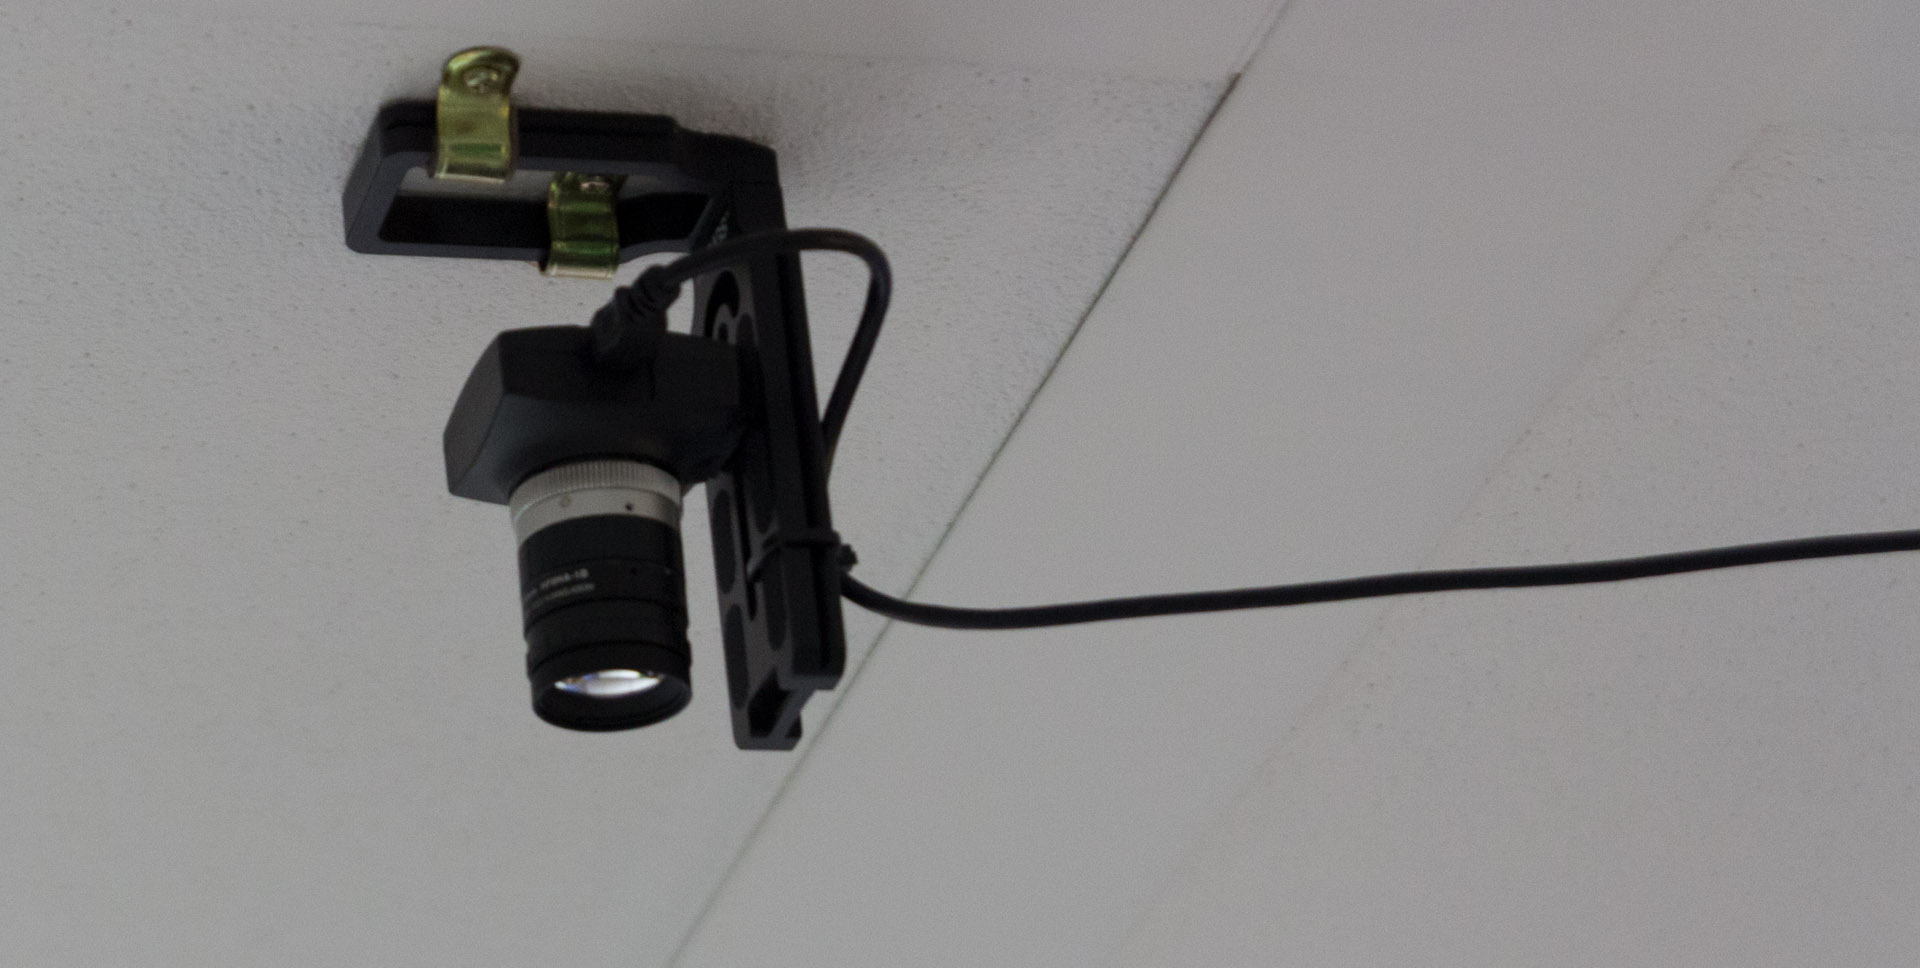
\includegraphics[width=4in]{Bilder/Eigene Fotos/IMG_0020.jpg}			
	\caption{Montage der uEye Camera.}
	\label{fig:uEyeMontage}
\end{figure}

\subsubsection{Unity Aufbau}\todo[inline, color=green]{Lukas}
\todo[inline, color=red]{Paul}
Der Teil des Systemaufbaus von \emph{MArC}, der sich vom Computer für die Ausführung der \emph{Unity}-Simulation (s. Abschnitt \ref{sec:UnityComp}) über die \emph{Leap Motion}, bis hin zur \emph{HTC Vive} erstreckt, ist ebenfalls in Abbildung~\ref{fig:AufbauMarc} dargestellt.\\
Die Verbindung von \emph{HTC Vive} zum Computer zur Ausführung der \emph{Unity}-Simulation wird sowohl per USB 2.0, als auch per HDMI 1.4 hergestellt. Über die HDMI-Verbindung werden die Bildschirme im \emph{HTC Vive} Head-Mounted-Display (HMD) als ein einzelnes Display auf dem verbundenen Computer eingebunden, genau so wie es auch mit einem normalen Bildschirm geschehen würde. Die USB 2.0 Verbindung des HMD dient hingegen dem Datenaustausch mit \emph{SteamVR}, welches auf dem Computer installiert ist.\\
Der \emph{Leap Motion} Controller wird über eine USB 3.0 Verbindung, welche per USB 2.0 Verlängerung angeschlossen ist, mit dem Computer verbunden. Dies ist deshalb problemlos möglich, weil die aktuelle Software des \emph{Leap Motion} Controllers die höhere Bandbreite der vorhandenen USB 3.0 Anbindung noch nicht ausnutzt, daher gibt \emph{Leap Motion} an, dass eine uneingeschränkte Nutzung an USB 2.0 möglich ist.~\cite{website:LeapMotionSupportQuestion}

\begin{figure}[H]
	\centering
	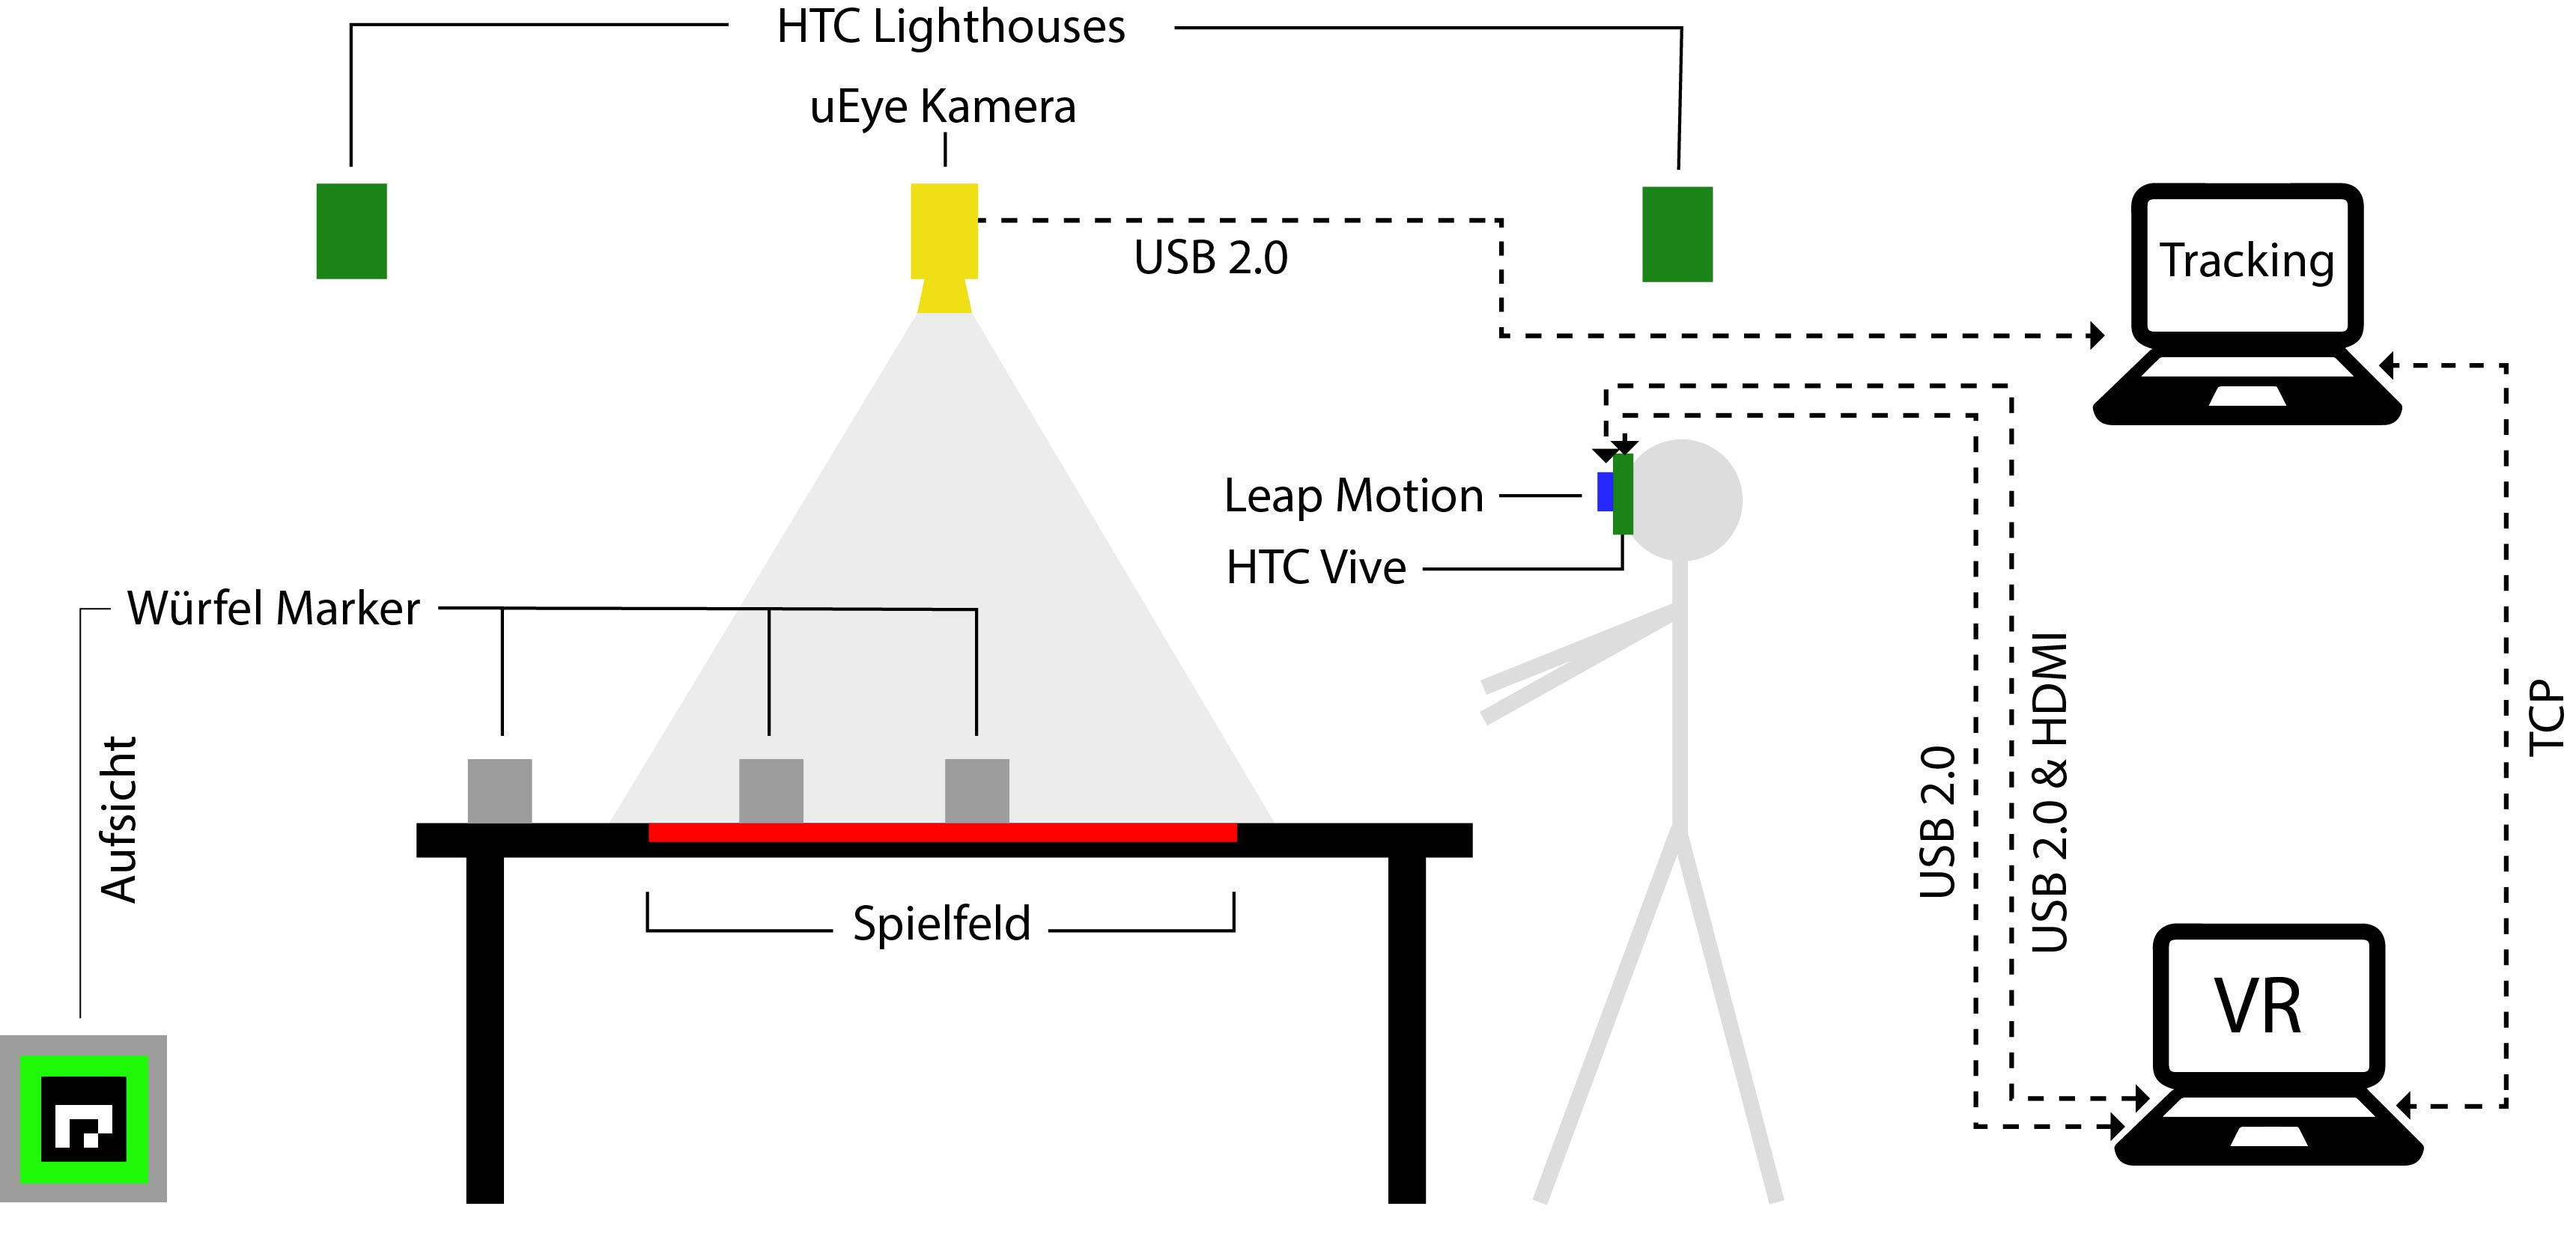
\includegraphics[width=\textwidth]{Bilder/Aufbau_MArC.jpg}
	\caption{Aufbau des \textit{MArC} Systems.}
	\label{fig:AufbauMarc}
\end{figure}


\subsection{Systemvoraussetzungen}\label{sec:sysVor}\todo[inline, color=green]{Lukas}
\todo[inline, color=red]{Paul}
Die Systemvoraussetzungen für \emph{MArC} sind in der ReadMe-Datei beschrieben, welche der im Projekt erstellten Software mitgeliefert ist. Die gesamte ReadMe-Datei ist in Abschnitt~\ref{sec:readMe} zu finden, außerdem enthält Abbildung~\ref{fig:marcReadMe} einen Ausschnitt der ReadMe-Datei, welcher die Voraussetzungen beschreibt, die vor dem Starten des Systems erfüllt sein müssen.

\begin{figure}
	\centering
	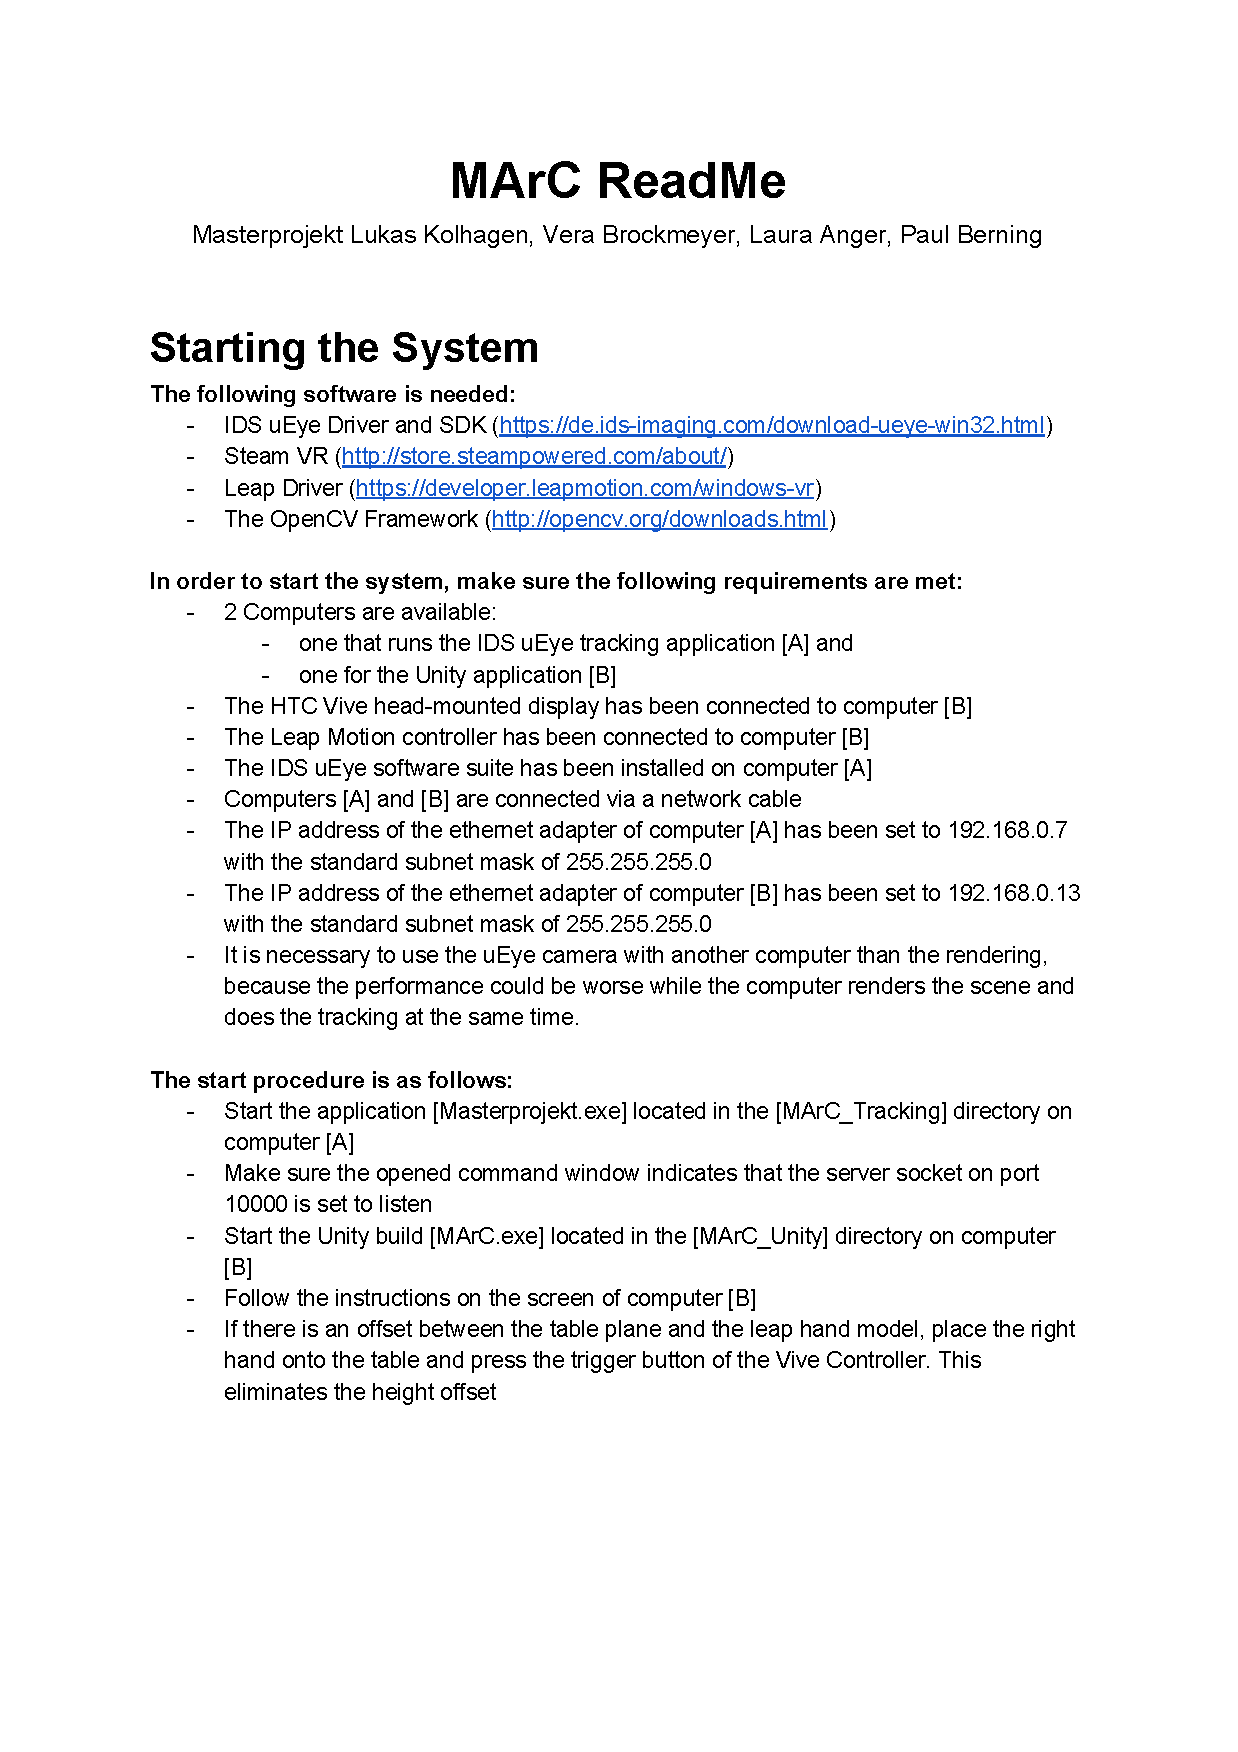
\includegraphics[page=1, trim=1cm 12.25cm 1cm 5.25cm, clip, width=\textwidth]{kapitel/anhang/ReadMe.pdf} 
	\caption{Auszug aus der \emph{MArC} ReadMe-Datei (vgl.~\ref{sec:readMe}).}
	\label{fig:marcReadMe}
\end{figure}

\subsection{Netzwerk}\label{sec:netzwerk}\todo[inline, color=green]{Lukas und Laura}
\todo[inline, color=red]{Paul}
Die in Kapitel \ref{sec:Winsock} beschriebene  \textcolor{red}{Winsocket} API stellt die Möglichkeit bereit, den Datentransport mittels TCP oder UDP zu verwenden. Für \emph{MArC} wurde ein TCP-Socket-Netzwerk bestehend aus (genau) einem Server und (genau) einem Client verwendet, weil der der in~\ref{sec:Netzwerk} beschriebene Fehlerschutz des TCP ausgenutzt werden sollte, um nicht manuell überprüfen zu müssen, ob Daten fehlerfrei übertragen wurden. Da die zu übertragende Datenmenge von \emph{MArC} hinreichend klein -- und von konstanter Größe -- ist, wurde die etwas höhere Geschwindigkeit durch den geringeren Overhead einer UDP-Socket-Verbindung als unnötig erachtet. \textcolor{red}{Kann man den Overhead prozentual angeben?} \\
In den beiden folgenden Abschnitten wird die Umsetzung der Netzwerk-Endpunkte an den beiden für \emph{MArC} verwendeten Computern beschrieben.
\subsubsection{Server-seitige Netzwerkanbindung}\label{sec:serverClient}\todo[inline, color=green]{Laura}
\todo[inline, color=blue]{Lukas}
\paragraph{Aufbauen der Netzwerkverbindung}
Da die Verbindung zwischen den beiden Rechnern per LAN-Kabel realisiert wurde, wird ein Server gestartet und eine Verbindung seitens des Clients ohne weitere Sicherheitsmechanismen erlaubt, so lange dieser den richtigen Port adressiert. Die entsprechenden Methoden stehen dank \textit{Winsock} (vgl. Abschnitt~\ref{sec:Winsock}) durch das Einbinden von \texttt{<winsock2.h>} und \texttt{<windows.h>} bereit und werden, wie in Quellcode-Auszug~\ref{lst:startTCPServer} (im Anhang einsehbar), verwendet. 

\paragraph{Datenübertragung}
Die Datenübertragen kann grob gesprochen in drei Teilbereiche unterteilt werden. Neben der bidirektionalen Übertragung von verschiedenen Status, müssen zum einen die Tracking-Daten der einzelnen sich im Arbeitsbereich befindlichen Objekte gesendet werden können und zum anderen die Positionen des Kalibrierungscontrollers während der Arbeitsbereichskalibrierung (vgl.Abschnitt Kapitel~\ref{sec:planeCalib} empfangen werden. \\

\lstinputlisting[title=\lstname, caption={\texttt{sendStatus()}-Methode in \texttt{TCP.cpp}}, label=lst:sendStatusVS, language={C++}, linerange=88-92, firstnumber=88]{Quellcode/TCP.cpp} 

Da die Übertragung der Status in beide Richtungen erfolgen muss, bedarf es einer Methode zum Senden (Quellcode-Auszug~\ref{lst:sendStatusVS})  und einer Methode zum Empfangen (Quellcode-Auszug~\ref{lst:receiveStatusVS}). Beide Methoden gehen von einem Status aus, der 4 Byte groß ist und sind ansonsten selbsterklärend. 

\lstinputlisting[title=\lstname, caption={\texttt{receiveStatus()}-Methode in \texttt{TCP.cpp}}, label=lst:receiveStatusVS, language={C++}, linerange=107-112, firstnumber=107]{Quellcode/TCP.cpp}

Die entsprechende Methode zum Versenden der Marker-Daten, also deren ID, Position, Winkel und Sichtbarkeits-Status, ist in Quellcode-Auszug \ref{lst:sendMarkerData} zu sehen. Alle eben genannten Eigenschaften eines Markers werden zu diesem Zweck in einem struct mit dem Namen \texttt{Marker\-Struct} (vgl. Quellcode-Auszug~\ref{lst:MarkerStruct}) gebündelt. 

\lstinputlisting[title=\lstname, caption={\texttt{sendMarkerData()}-Methode in \texttt{TCP.cpp}}, label=lst:sendMarkerData, language={C++}, linerange=99-103, firstnumber=99]{Quellcode/TCP.cpp} 

Der Vollständigkeit halber befindet sich im Anhang der Quellcode-Auszug~\ref{lst:getPointerOfMarkerVec} der \texttt{get\-Pointer\-Of\-Marker\-Vec()}-Methode. Diese dient im Wesentlichen zur Umsortierung der entsprechenden Daten aus dem umfangreicheren \texttt{allMarkers}-Array in das \texttt{Marker\-Struct}-Array. Damit wird dafür gesorgt, dass nur die relevanten Daten übertragen werden. 

\lstinputlisting[title=\lstname, caption={\texttt{MarkerStruct} in \texttt{TCP.h}}, label=lst:MarkerStruct, language={C++}, linerange=13-20, firstnumber=13]{Quellcode/TCP.h} 

Während der Kalibrierung des Arbeitsbereichs (vgl. Kapitel~\ref{sec:planeCalib}) wird die Position des Kalibrierungscontrollers nach jedem Auslösen des Triggers von der \textit{Unity}-Simulation an die Tracking-Anwendung gesendet. Die entsprechende Methode zum Empfangen der dreidimensionalen Position in Unitykoordinaten ist in Quellcode-Auszug~\ref{lst:receiveControllerPositions} abgebildet. Neben dem reinen Empfang der Daten, der äquivalent zu der \texttt{receive\-Status()}-Methode funktioniert, werden hier die ankommenden Daten aus dem Array in einen anderen Datentyp konvertiert, um eine Weiterverarbeitung während der Arbeitsbereichskalibrierung zu vereinfachen. 

\lstinputlisting[title=\lstname, caption={\texttt{receiveControllerPositions()}-Methode in \texttt{TCP.cpp}}, label=lst:receiveControllerPositions, language={C++}, linerange=116-125, firstnumber=116]{Quellcode/TCP.cpp}




\subsubsection{Client seitige Netzwerkanbindung}\todo[inline, color=green]{Lukas}
\todo[inline, color=red]{Laura}
\paragraph{Aufbauen der Netzwerkverbindung}
Das Aufbauen der Netzwerkverbindung vom Client zum Server, also von der \textit{Unity}-Simulation zur Tracking-Anwendung, geschieht mit Hilfe der von Winsock (vgl. Abschnitt~\ref{sec:Winsock}) bereitgestellten Klasse \texttt{System.Net.Sockets.TcpClient} wie in Quellcode-Auszug~\ref{lst:setupSocket} dargestellt. Die Netzwerkverbindung wird zu einer fest vorgegebenen IP-Adresse hergestellt.

\lstinputlisting[title=\lstname, caption={\texttt{setupSocket()}-Methode in \texttt{readInNetWorkData.cs}}, label=lst:setupSocket, language={[Sharp]C}, linerange=69-79, firstnumber=69]{Quellcode/readInNetworkData.cs}

\paragraph{Datenübertragung}
Nach einer erfolgreich hergestellten Verbindung sieht das Netzwerkmodul in \emph{MArC} sowohl eine Übertragung von verschiedenen Status zur Steuerung des Programmablaufs, als auch die Übetragung der Positionen des Kalibrierungscontrollers während der Arbeitsbereichskalibrierung (vgl. Kapitel~\ref{sec:planeCalib}) sowie die Übertragung der Tracking-Daten für die Simulation vor.

Die Übertragung einer Position des \emph{HTC Vive}-Controllers während der Arbeitsbereichskalibrierung wird durch das Drücken der \emph{Trigger}-Taste am Controller ausgelöst. Dadurch wird die Methode \texttt{setPosition()} in \texttt{TableCalibration.cs} mit der aktuellen Position des Controllers in Unitykoordinaten als Übergabewert aufgerufen. Von dort werden bei erfolgreicher Beendigung der Kalibrierung die vier Eckpunkte des Arbeitsbereichs abgespeichert und an \texttt{ca\-li\-bra\-tion\-Done()} in \texttt{set\-up\-Scene.cs} weitergegeben. In \texttt{setupScene.cs} werden diese Positionen verwendet, um den Arbeitsbereich für den Benutzer zu kennzeichnen. Dies wird in Abschnitt~\ref{sec:planeCalib} beschrieben.

\lstinputlisting[title=\lstname, caption={\texttt{sendTCPstatus()}-Methode in \texttt{readInNetWorkData.cs}}, label=lst:sendStatus, language={[Sharp]C}, linerange=81-89, firstnumber=81]{Quellcode/readInNetworkData.cs}

Das Senden und Empfangen von Status seitens der Unity-Simulation ist in den Quellcode-Auszügen~\ref{lst:sendStatus} und~\ref{lst:receiveStatus} dargelegt. Die Methode zum Senden eines Status ist selbsterklärend. Die \texttt{receiveTCPstatus()}-Methode prüft zunächst, ob eine Netzwerkverbindung hergestellt, also das Socket bereit ist. Anschließend werden genau vier Bytes vom Netzwerk-Datenstrom gelesen, als 32-Bit-Integer interpretiert und zurückgegeben.

\lstinputlisting[title=\lstname, caption={\texttt{receiveTCPstatus()}-Methode in \texttt{readInNetWorkData.cs}}, label=lst:receiveStatus, language={[Sharp]C}, linerange=91-106, firstnumber=91]{Quellcode/readInNetworkData.cs}

Das Empfangen und Interpretieren der Tracking-Daten, nachdem die Simulation gestartet wurde, gestaltet sich ein wenig komplexer und ist im Quellcode-Auszug~\ref{lst:interpretData} aufgeführt. Der Auszug wurde aus Platzgründen in den Anhang verschoben.\\
In der Methode \texttt{interpretTCPMarkerData()} wird ein Byte-Puffer konstanter Länge, welcher vorher vom Netzwerk-Datenstrom gelesen wurde, dahingehend interpretiert, dass anschließend die Daten für alle aktiven Tracking-Marker in geeigneter Form zur weiteren Verarbeitung vorliegen. Als geeignete Form ist hier die Klasse \texttt{Marker} zu nennen, welche als Attribute die ID, die X- und Y-Position, den Winkel und den Status des jeweiligen Markers enthält.\\ 
Beim Interpretieren der Marker werden zunächst die ersten vier Bytes an der von der Schleife abhängigen Pufferposition als ID interpretiert. Sofern die ID gleich $-1$ ist, wird der aktuelle Schleifendurchlauf beendet, da dieser Marker nicht aktiv (valide) ist. Sollte die ID gleich $-2$ sein, indiziert dies, dass für das aktuelle Frame alle Marker übertragen wurden und die Schleife abgebrochen werden kann. In allen anderen Fällen ist die ID valide und alle zusätzlichen Eigenschaften des Markers werden aus dem Puffer gelesen und über den BitConverter geeignet interpretiert. Zuletzt wird ein global angelegtes \texttt{Marker}-Array in jedem Schleifendurchlauf mit dem verarbeiteten Marker befüllt. Bei anschließendem Rendern der Simulation wird dann nur noch auf die so aufbereiteten Daten~--~und nicht mehr auf die Netzwerkdaten~--~zugegriffen.

\subsection{Starten des Systems}\todo[inline, color=green]{Lukas}
\todo[inline, color=red]{Laura}
Nachdem sichergestellt wurde, dass alle in~\ref{sec:sysVor} beschriebenen Voraussetzungen bestehen, kann das System gestartet werden, indem zunächst die Tracking-Anwendung (auf dem einen Computer, vgl.~\ref{sec:TrackingComp}) und anschließend die aus Unity heraus erstellte Anwendung (auf dem anderen Computer, vgl.~\ref{sec:UnityComp}) gestartet wird. Auf letzterem Computer beginnt darauffolgend die Menüführung, welche in \ref{sec:menu} beschrieben ist. \textcolor{red}{War es nicht so, dass doPoseCalibInVS (oder war es SelectCalibrationTarget) gar nicht angezeigt werde konnte? Wäre zu überlegen das dann raus zu lassen.}
\subsection{Menüführung}\label{sec:menu}\todo[inline, color=green]{Lukas}
\todo[inline, color=red]{Laura}
Die Menüführung dient dazu, den Benutzer durch alle notwendigen Schritte zu leiten, die vor dem Starten der eigentlichen Simulation erforderlich sind. Im nachfolgenden Abschnitt~\ref{sec:menus} werden alle verfügbaren Menüs der Anwendung aufgelistet und kurz beschrieben, während im Abschnitt~\ref{sec:menuAblauf} der Ablauf der Menüführung erläutert wird.


\subsubsection{Menüs}\label{sec:menus}\todo[inline, backgroundcolor=green]{Lukas und Laura}
\todo[inline, color=red]{Laura}
Die folgenden Menüs sind Bestandteil der Menüführung:

\begin{minipage}{0.6\textwidth}
	\begin{figure}[H] 
		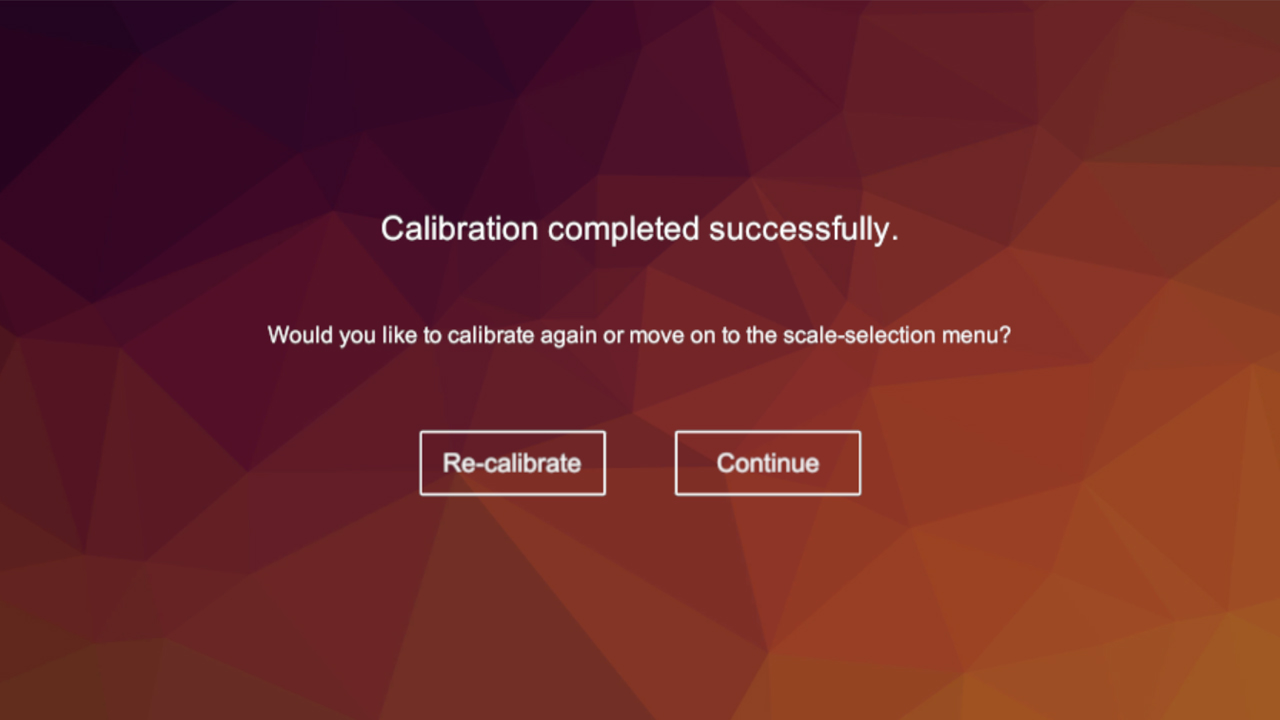
\includegraphics[trim=3cm 2cm 3cm 2cm, clip, width=0.9\textwidth]{Bilder/CalibDone.jpg}
			\label{fig:CalibDone}
	\end{figure}
\end{minipage}
\begin{minipage}{0.4\textwidth}
	\texttt{CalibDone}:\\
	Wird aufgerufen, wenn die Kalibrierung des Arbeitsbereichs abgeschlossen ist. Es informiert den Benutzer, dass die Kalibrierung erfolgreich war und der Vorgang fortgesetzt werden kann. Zusätzlich wird die Option geboten, erneut zu kalibrieren.
\end{minipage}\\

\begin{minipage}{0.6\textwidth}
	\begin{figure}[H] 
		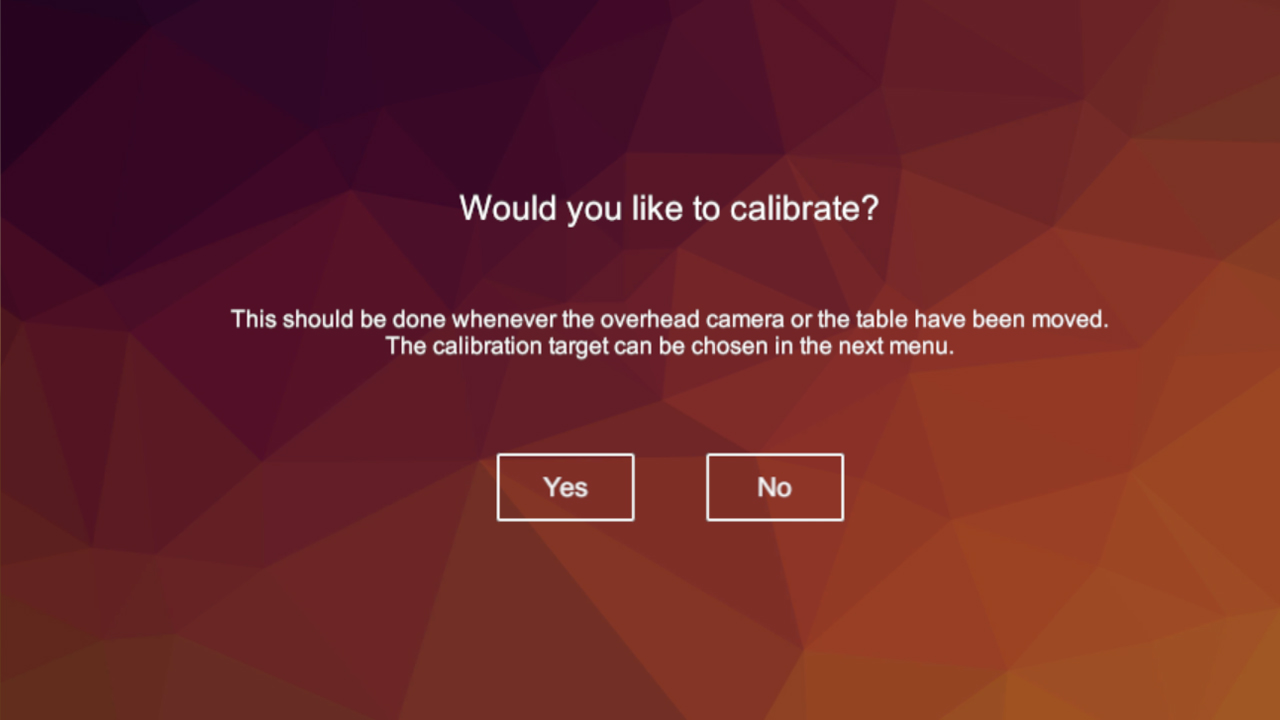
\includegraphics[trim=3cm 2cm 2cm 2cm, clip, width=0.9\textwidth]{Bilder/CalibrateOrNot.jpg}
			\label{fig:CalibrateOrNot}
	\end{figure}
\end{minipage}
\begin{minipage}{0.4\textwidth}
	\texttt{CalibrateOrNot}:\\
	Erscheint nach dem Verlassen des \texttt{Welcome}-Menüs und erlaubt dem Benutzer eine Kalibrierung durchzuführen oder eine bereits durchgeführte Kalibrierung zu laden.
\end{minipage}\\

\begin{minipage}{0.6\textwidth}
	\begin{figure}[H] 
		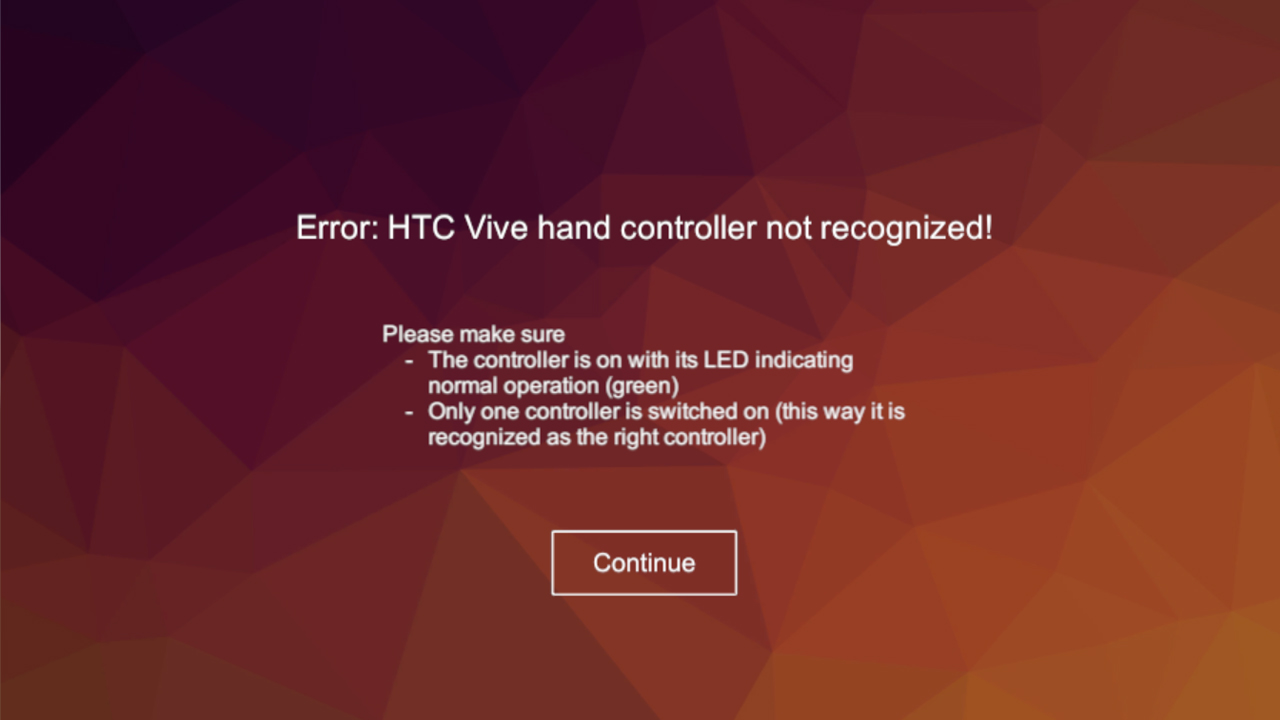
\includegraphics[trim=3cm 1cm 3cm 3cm, clip, width=0.9\textwidth]{Bilder/ControllerNotFound.jpg}
			\label{fig:ControllerNotFound}
	\end{figure}
\end{minipage}
\begin{minipage}{0.4\textwidth}
	\texttt{ControllerNotFound}:\\
	Warnt den Benutzer nach dem Starten der Kalibrierung, dass der \textit{HTC Vive}-Controller, welcher für die Kalibrierung benötigt wird, nicht eingeschaltet ist. Während das Menü angezeigt wird, kann der Benutzer den Controller einschalten und anschließend auf \texttt{Continue} klicken.
\end{minipage}\\

\begin{minipage}{0.6\textwidth}
	\begin{figure}[H] 
		\includegraphics[trim=3cm 1cm 3cm 3cm, clip, width=0.9\textwidth]{Bilder/doPlaneCalibInVS.jpg}
			\label{fig:doPlaneCalibInVS}
	\end{figure}
\end{minipage}
\begin{minipage}{0.4\textwidth}
	\texttt{doPlaneCalibInVS}:\\
	Dient dem Benutzer als Anleitung für die Durchführung der Kalibrierung des Arbeitsbereichs. Diese wird in \ref{sec:planeCalib} genauer beschrieben.
\end{minipage}\\

\begin{minipage}{0.6\textwidth}
	\begin{figure}[H] 
		\includegraphics[trim=3cm 2cm 3cm 2cm, clip, width=0.9\textwidth]{Bilder/doPoseCalibInVS.jpg}
			\label{fig:doPoseCalibInVS}
	\end{figure}
\end{minipage}
\begin{minipage}{0.4\textwidth}
	\texttt{doPoseCalibInVS}:\\
	Dient dem Benutzer als Anleitung für die Durchführung der Kamera-Kalibrierung. Diese wird in \ref{sec:camCalib} genauer beschrieben.
\end{minipage}\\

\begin{minipage}{0.6\textwidth}
	\begin{figure}[H] 
		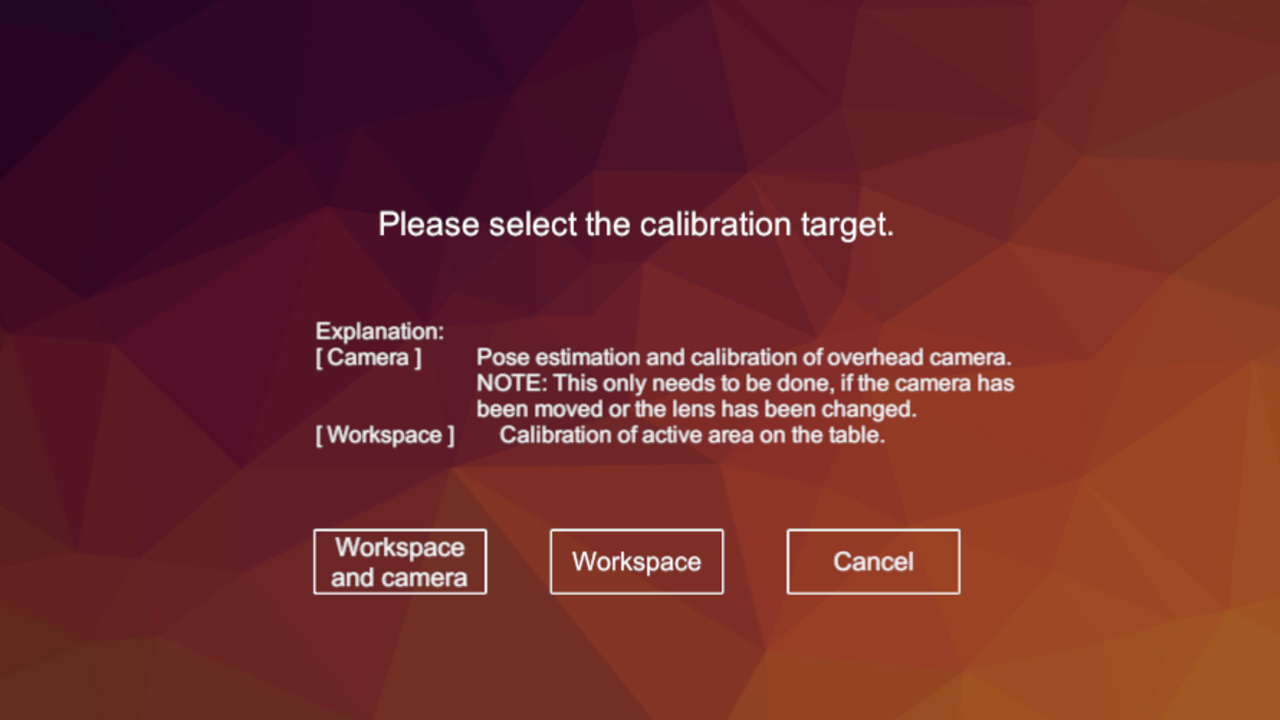
\includegraphics[trim=3cm 1cm 3cm 3cm, clip, width=0.9\textwidth]{Bilder/SelectCalibrationTarget.jpg}
			\label{fig:SelectCalibrationTarget}
	\end{figure}
\end{minipage}
\begin{minipage}{0.4\textwidth}
	\texttt{SelectCalibrationTarget}:\\
	Erlaubt die Auswahl der Art der Kalibrierung. Es kann hier entweder nur der Arbeitsbereich oder sowohl der Arbeitsbereich, als auch die Kamera kalibriert werden. Die Kalibrierung ist näher in \ref{sec:calib} beschrieben.
\end{minipage}\\

\begin{minipage}{0.6\textwidth}
	\begin{figure}[H] 
		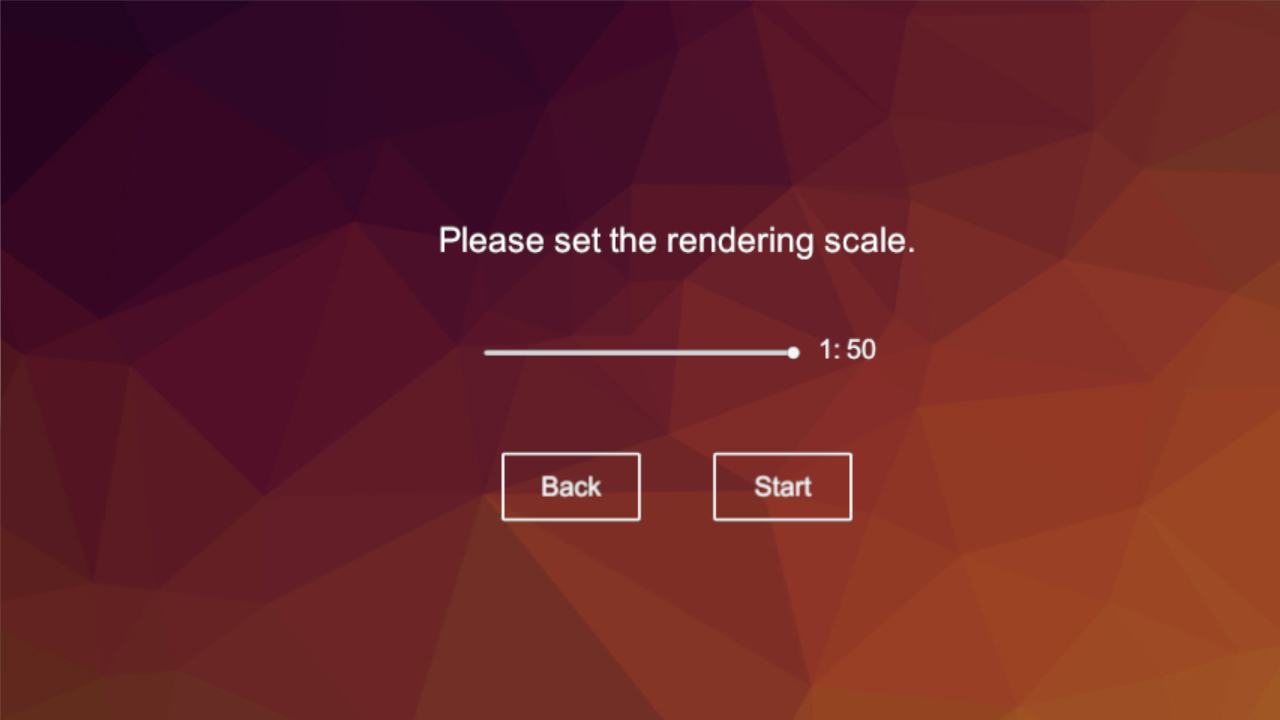
\includegraphics[trim=3.5cm 1cm 2.5cm 3cm, clip, width=0.9\textwidth]{Bilder/SetScale.jpg}
			\label{fig:SetScale}
	\end{figure}
\end{minipage}
\begin{minipage}{0.4\textwidth}
	\texttt{SetScale}:\\
	Stellt das letzte Menü vor dem Starten der Simulation dar. In diesem kann der Benutzer den Maßstab der Gebäudesimulation einstellen und anschließend die Simulation starten.
\end{minipage}\\

\begin{minipage}{0.6\textwidth}
	\begin{figure}[H] 
		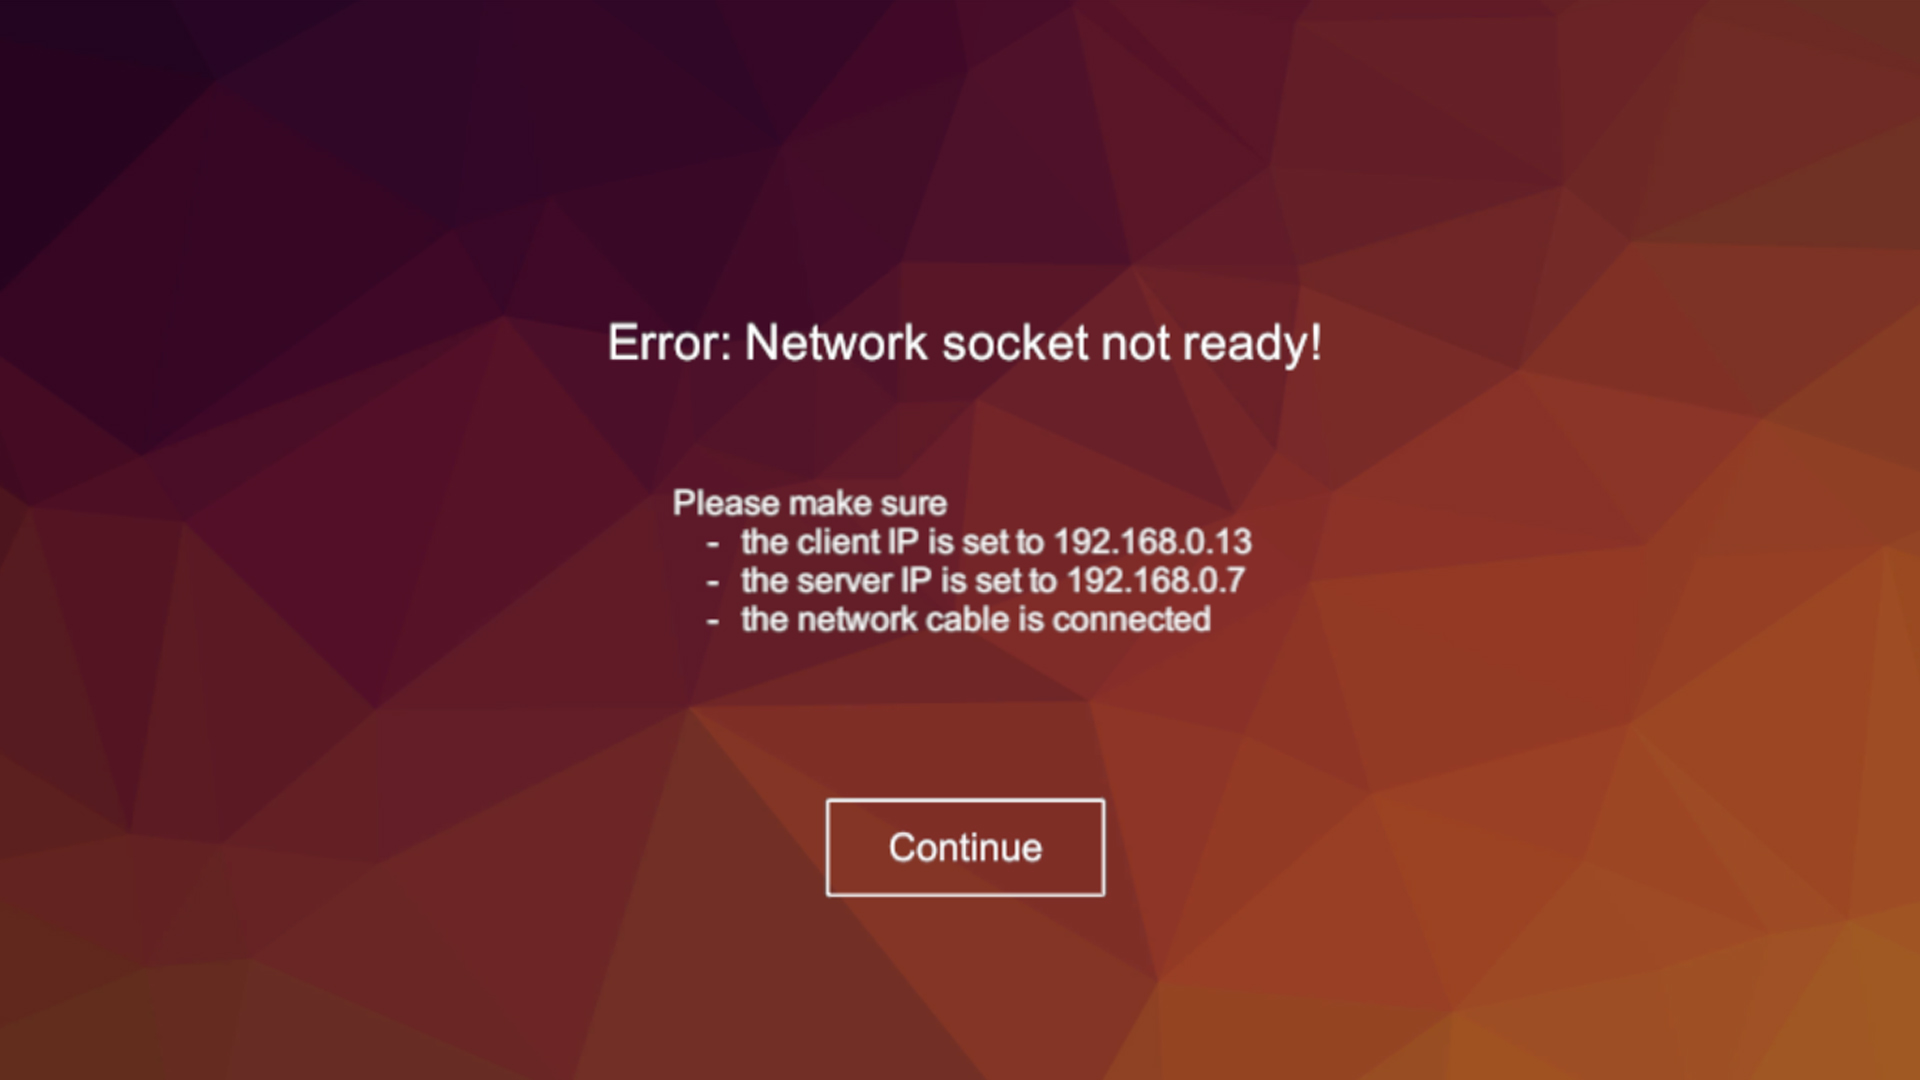
\includegraphics[trim=3cm 1cm 3cm 3cm, clip, width=0.9\textwidth]{Bilder/SocketNotReady.jpg}
			\label{fig:SocketNotReady}
	\end{figure}
\end{minipage}
\begin{minipage}{0.4\textwidth}
	\texttt{SocketNotReady}:\\
	Warnt den Benutzer nach dem Verlassen des \texttt{Welcome}-Menüs, dass die Netzwerkverbindung zwischen den beiden Computern nicht bereit ist. Nach Bestätigung dieses Hinweises durch einen Klick auf \texttt{Continue}, kehrt der Benutzer zum \texttt{Welcome}-Menü zurück. %Anschließend kann der Vorgang fortgesetzt werden, wenn die Netzwerkverbindung hergestellt wurde. Andernfalls erscheint wieder \texttt{SocketNotReady}.
\end{minipage}\\

\begin{minipage}{0.6\textwidth}
	\begin{figure}[H] 
		
\includegraphics[trim=3cm 2cm 3cm 2cm, clip, width=0.9\textwidth]{Bilder/Welcome.jpg}
			\label{fig:Welcome}
	\end{figure}
\end{minipage}
\begin{minipage}{0.4\textwidth}
	\texttt{Welcome}:\\
	Erscheint als erstes Menü. Hier erhält der Nutzer eine kurze Information darüber, wie die Anwendung heißt und wozu sie dient.
\end{minipage}\\

\subsubsection{Ablauf der Menüführung}\label{sec:menuAblauf}\todo[inline, color=green]{Lukas}
\todo[inline, color=red]{Laura}
Der Ablauf der Menüführung von \textit{MArC} ist in Abbildung~\ref{fig:menuFlow} dargestellt. Die einzelnen Menüs sind bereits in~\ref{sec:menus} beschrieben worden.

\begin{figure}[htbp]
	\centering
	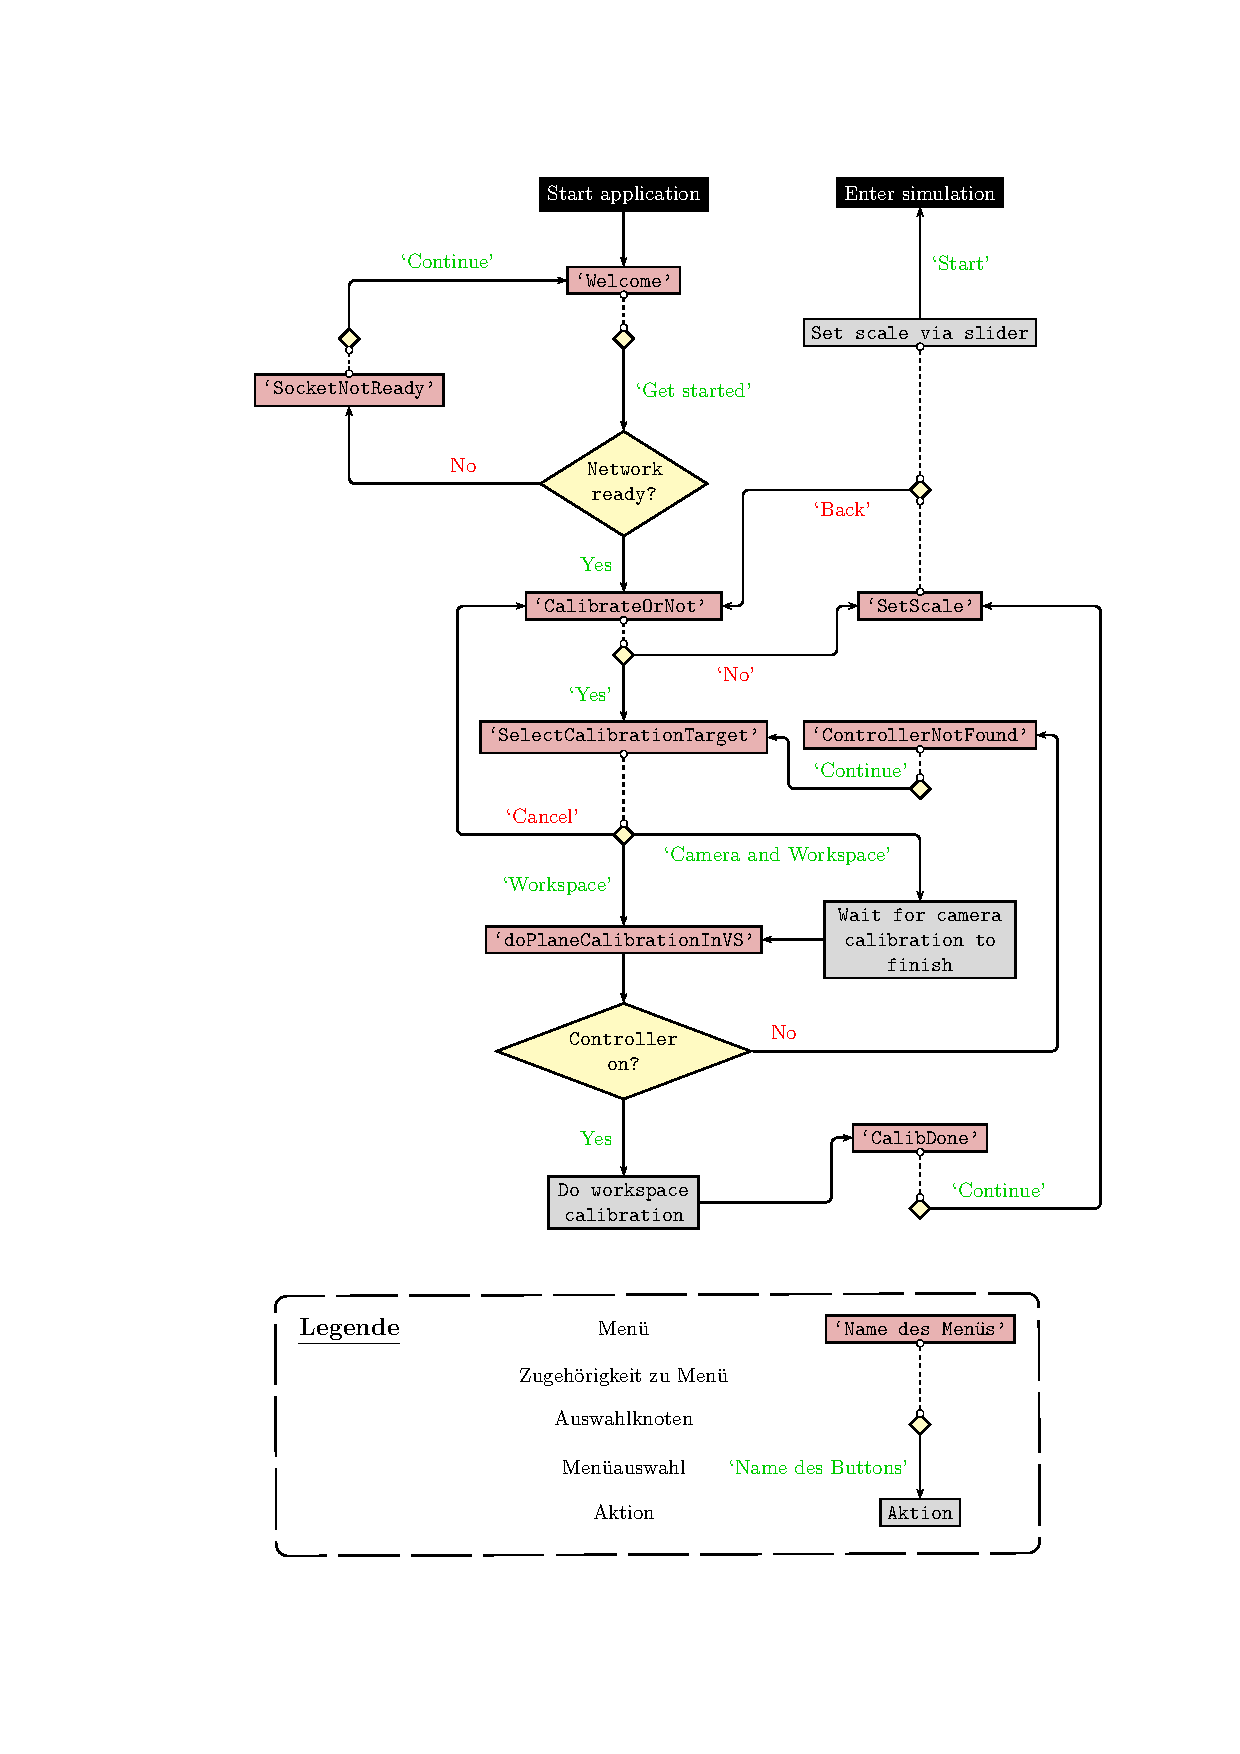
\includegraphics[scale=.9, trim=5.5cm 2.5cm 3.5cm 2.5cm]{kapitel/system/MP_Menu_Flowchart.pdf}
	\caption{Flussdiagramm der Menüführung.}
	\label{fig:menuFlow}
\end{figure}

Nach dem Starten der Anwendung wird zunächst das Menü \texttt{Welcome} angezeigt. Dieses enthält nur einen Button \textit{Get started}. Sobald dieser gedrückt wird, prüft die Anwendung, ob eine Netzwerkverbindung zu dem Computer mit der Tracking-Anwendung besteht. Sollte dies nicht der Fall sein, wird das Menü \texttt{Socket\-Not\-Ready} angezeigt. Dieses verlässt der Benutzer über einen Klick auf \texttt{Continue}, anschließend wird erneut das Menu \texttt{Welcome} angezeigt. Wenn zu diesem Zeitpunkt die Netzwerkverbindung korrekt hergestellt wurde, gelangt der Benutzer zum Menü \texttt{Calibrate\-Or\-Not}, anderenfalls wird wiederholt \texttt{Socket\-Not\-Ready} angezeigt.

In \texttt{CalibrateOrNot} hat der Benutzer die Auswahl zwischen den Schaltflächen \textit{Yes} und \textit{No}. Bei einem Klick auf \textit{Yes} wird anschließend \texttt{Select\-Calibration\-Target} angezeigt, bei einem Klick auf \textit{No} lädt das System eine zuvor durchgeführte Kalibrierung und das Menü \texttt{Set\-Scale} wird geöffnet.

\texttt{Select\-Calibration\-Target} stellt den Benutzer vor die Wahl entweder nur den Arbeitsbereich (\textit{Work\-space}) oder sowohl den Arbeitsbereich als auch die Kamera zu kalibrieren (\textit{Camera and Workspace}). Außerdem besteht die Möglichkeit über \textit{Cancel} zum Menü \texttt{Calibrate\-Or\-Not} zurückzukehren.

Wählt der Benutzer \textit{Camera and Workspace} in \texttt{Select\-Calibration\-Target} aus, so informiert die Anwendung die Tracking-Anwendung auf dem anderen Computer und wartet anschließend darauf, dass von dort die Bestätigung gesendet wird, dass die Kamerakalibrierung abgeschlossen ist. Anschließend wird das Menü \texttt{doPlane\-Calibration\-InVS} angezeigt, welches auch aufgerufen wird, wenn der Benutzer \textit{Work\-space} in \texttt{Select\-Calibration\-Target} wählt.

Im Menü \texttt{doPlane\-Calibration\-InVS} wird zunächst geprüft, ob der für die Kalibrierung notwendige \textit{HTC Vive}-Controller eingeschaltet ist. Sollte dies nicht der Fall sein, wird \texttt{Controller\-Not\-Found} aufgerufen. Dieses kann mit einem Klick auf \textit{Continue} verlassen werden, woraufhin wieder \texttt{Select\-Calibration\-Target} angezeigt wird.\\
Sofern der \textit{HTC Vive}-Controller beim Aufruf von \texttt{doPlane\-Calibration\-InVS} eingeschaltet ist, wird nach Durchführung der Kalibrierung des Arbeitsbereichs das Menü \texttt{CalibDone} angezeigt.

\texttt{Calib\-Done} kann über einen Klick auf \textit{Continue} verlassen werden und führt den Nutzer anschließend zu \texttt{SetScale}. Aus diesem Menü kann über den Button \textit{Back} entweder zu \texttt{CalibrateOrNot} zurückgekehrt oder die Simulation, mit dem im Menü über den Slider eingestellten Maßstab, gestartet werden.



\subsection{Kontextmenü}\label{sec:kontextMenu}\todo[inline, color=green]{Laura und Lukas}
\todo[inline, color=red]{Paul}
Die virtuellen Objekte, die den in Kapitel~\ref{sec:WürfelMarker} beschriebenen Aluminiumwürfeln zugeordnet werden, sind zunächst würfelförmig und können zur Laufzeit der Anwendung vom Benutzer verschoben, rotiert und skaliert werden.\textcolor{red}{Diese virtuellen Objekte repräsentieren bei MArC die Gebäude}.  Die Verschiebung und Rotation kann über eine entsprechende Veränderung der Lage des realen Marker-Würfels geschehen. Für die Skalierung kann wie in Kapitel~\ref{sec:KontextMenuSwitch} beschrieben das sogenannte Kontextmenü aufgerufen werden. Dieses beinhaltet neben den Marker Handles (vgl. Kapitel~\ref{sec:markerHandles}) zur dreidimensionalen Skalierung des virtuellen Objekts auch eine Art Übersichtstafel der Gebäudeeigenschaften des zugehörigen virtuellen Markers. Beispiele für Letzteres sind in Abbildung~\ref{fig:KontextmenuExamples} zu sehen. Im Folgenden wird, wenn nicht anders erwähnt, die Übersichtstafel mit \glqq Kontextmenü\grqq{} bezeichnet. Die Idee des Kontextmenüs ist aus dem Treffen mit den Mitarbeitern eines Architekturbüros zu Beginn des Projektes entstanden (vgl. Abschnitt \ref{sec:problemanalyse}). Diese hatten eine detaillierte Beschreibung der einzelnen Gebäude als sinnvoll und nützlich für die Umsetzung einer Anwendung wie den \textit{MArC} beschrieben.\\
Da zu Beginn der Anwendung im \texttt{SetScale}-Menü (vgl. Kapitel~\ref{sec:menuAblauf}) der Maßstab der Architekturszene vom Benutzer ausgewählt wird und zusätzlich wie beschrieben eine Skalierung der einzelnen Objekte durchgeführt werden kann, muss sich der Inhalt des Kontextmenüs dynamisch ändern können. Die dazu notwendigen Berechnungen der Gebäudeeigenschaften sind in Kapitel~\ref{sec:KontextMenuInhalt} erläutert. 

\begin{figure}[H]
	\centering
	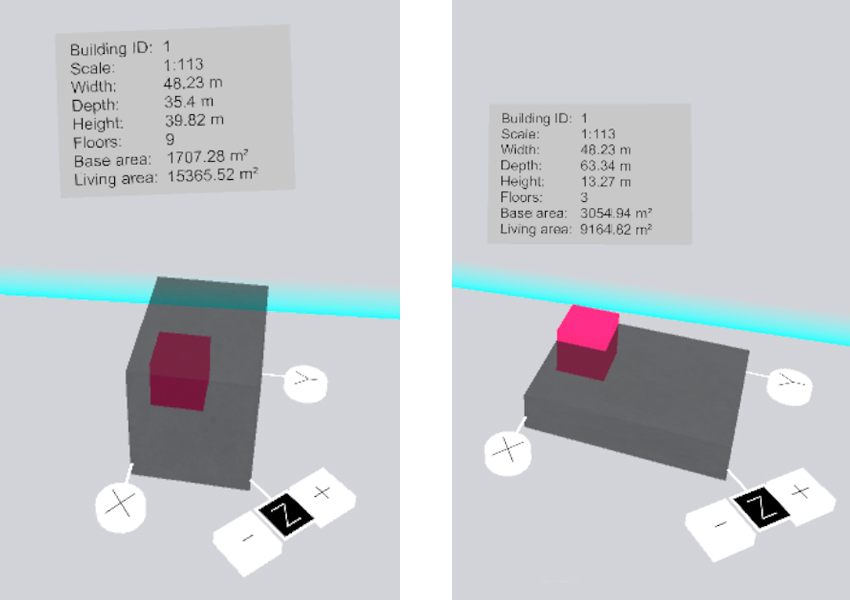
\includegraphics[scale=.3]{Bilder/Eigene Fotos/KontextMenue.jpg}
	\caption{Zwei Beispiele für ein Kontextmenü eines Würfels mit ID 1.}
	\label{fig:KontextmenuExamples}
\end{figure}

\subsubsection{Marker Handles}\label{sec:markerHandles}\todo[inline, color = green]{Paul}
\todo[inline, color=blue]{Lukas}
Jeder Marker verfügt über die Möglichkeit in seiner Größe in X-, Y- und Z-Achse verändert zu werden. Diese sog. \glqq Handles\grqq{} sind sichtbar, wenn das Kontextmenü angezeigt wird (s. Abschnitt  \ref{sec:kontextMenu}. Die Handles bestehen aus Zylindern, die mit einem Collider versehen wurden. Die X- und Y- Achse wird betätigt, indem der Benutzer mit einem Finger das jeweiligen Handle berührt und dann in die entsprechende Richtung zieht. Die Größe in Z-Achse wird über \glqq+\grqq{} und \glqq-\grqq Button gesteuert. Drückt der Benutzer diese Buttons, wird das Gebäude um je ein Stockwerk erhöht oder verniedrigt. \\

Die Interaktion der Handles mit der Hand des Nutzers wurde über das Leap- Handmodell umgesetzt; dieses besitzt Collider, die an den Fingern des Modells angebracht sind und sich simultan mit der Hand des Nutzers bewegen. Berührt die Hand nun einen der Handler, wird dieser Collider des Handlers "angesprochen". Im Falle der X-, und Y-Handles wird in der \texttt{update} Funktion des Skripts \texttt{contextMenuTrigger.cs} ein Vektor berechnet, der die Start und Endposition der Bewegung miteinander verrechnet. Im Falle einer Bewegung in X Position wird die sog. \glqq localDifference\grqq{} berechnet, dies ist der Abstand des Fingers zur Position des Markers. Die eigentliche Skalierung wird dann wie folgt berechnet:\\

 \begin{lstlisting}
pos = (startPosition.x - localDifference.y) / 2, startPosition.y, startPosition.z)
 \end{lstlisting}

Das Gebäude wird dann um den Vektor pos im lokalen Objektkoordinatensystem vergrößert.\\
Für die Bewegung in Y berechnet sich der Vektor wie folgt:

 \begin{lstlisting}
pos = (startPosition.x , startPosition.y, (startPosition.z - localDifference.y) / 2)
 \end{lstlisting}

Es fällt auf, dass in der zu verändernden Achse verschiedene Achsen zur Berechnung verwendet werden müssen. Dies kommt daher, dass das Koordinatensystem der Leap Motion nicht equivalent zu dem in Unity ist.\\
Dass der Wert der zu verändernden Achse halbiert wird, hat sich empirisch als Sinnvoll herausgestellt. Ohne diese "Übersetzung" der Bewegung würde das Gebäude nicht equivalent zur Fingerbewegung vergrößert oder verkleinert werden. 

\subsubsection{Ein- und Ausblenden des Kontextmenüs} \label{sec:KontextMenuSwitch}\todo[inline, color=green]{Lukas}
\todo[inline, color=red]{Paul}
Zum Ein- und Ausblenden des in Abschnitt~\ref{sec:kontextMenu} beschriebenen Kontextmenüs wird sich der Interaktionsmechanismen des \emph{Leap Motion} Controllers bedient.\\
Zum Öffnen des Kontextmenüs muss der Benutzer mit einer vom \emph{Leap Motion} Controller erkannten Hand die obere Fläche eines Markers berühren. Diese Interaktion funktioniert über einen in \emph{Unity} erstellten Collider, welcher quaderförmig ist und in der Mitte eines jeden Markers nach oben herausschaut (vgl. Abb.~\ref{fig:KontextmenuCollider}). Sobald ein Teil der Hand des Benutzers in diesem Collider eindringt, wird in der Methode \texttt{OnTriggerEnter()} im Skript \texttt{contextMenuTrigger.cs} das Kontextmenü (dessen \emph{GameObject} dort \texttt{CanvasTransform} heißt) sowie die in Abschnitt~\ref{sec:markerHandles} beschriebenen Marker Handles aktiviert.\\
Auf die gleiche Weise wird das Kontextmenü mit den Marker Handles auch wieder geschlossen, wenn nämlich der Benutzer bei geöffnetem Kontextmenü die obere Fläche des Markers berührt. Dann werden die zum Kontextmenü gehörigen \emph{GameObjects} wieder deaktiviert.

\begin{figure}
	\centering
	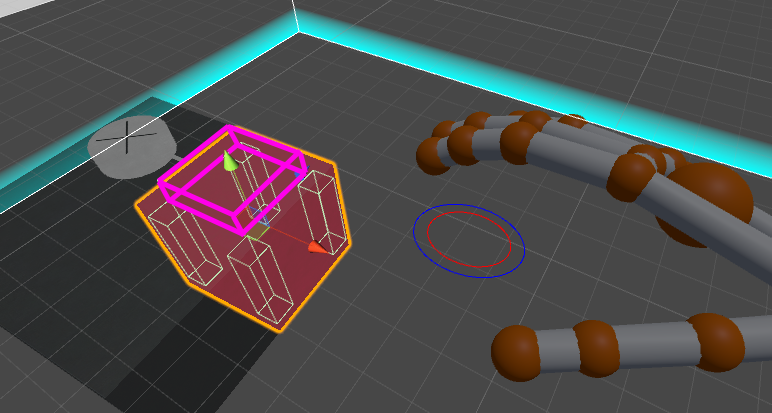
\includegraphics[width=\textwidth]{Bilder/Contextmenu_Collider}
	\caption{Collider zum Ein- und Ausblenden des Kontextmenüs (in Pink eingefärbt).}
	\label{fig:KontextmenuCollider}
\end{figure}

\subsubsection{Berechnung der Gebäudeeigenschaften} \label{sec:KontextMenuInhalt}\todo[inline, color=green]{Laura}
\todo[inline, color=blue]{Lukas}
Wie auf Abbildung \ref{fig:standardMarker} zu sehen, enthält das Kontextmenü neben der Anwendungsspzfischen ID des jeweiligen Gebäudes, noch eine Reihe weiterer Informationen über dieses.  Zunächst wird der Maßstab, den der Benutzer zu Beginn der Anwendung im \texttt{setScale}-Menü (vgl. Abschnitt \ref{sec:menuAblauf}) auswählen kann, angegeben. Wenn das Objekt nicht bereits durch den Benutzer anhand der Handles transformiert wurde, sieht es aus wie auf der bereits erwähnten Abbildung \ref{fig:standardMarker}. Diese zeigt einen Standard-Marker mit 4 Geschossen. Über den z-Handle (vgl. Abschnitt \ref{sec:markerHandles}) können einzelne Geschosse hinzugefügt oder gelöscht werden. Was im Kontextmenü zum einen natürlich direkten Einfluss auf die Geschossigkeit hat und zum anderen zur Veränderung der Höhe des jeweiligen Gebäudes führt. Neben der Höhe sind die Breite und Höhe, sowie die Grund- und Wohnfläche von der Skalierung des virtuellen Markers abhängig. Alle im Kontextmenü dargestellten Größen, bis auf die ID und die Geschossigkeit sind von dem ebenfalls dort aufgeführten und bereits erwähnten Maßstab abhängig. 

\begin{figure}
	\centering
	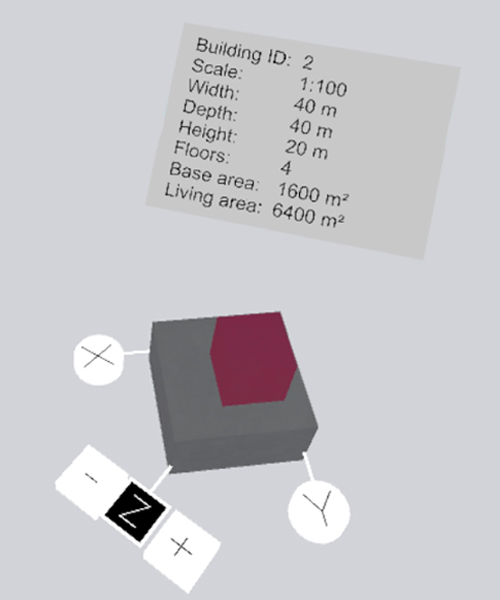
\includegraphics[scale=.3]{Bilder/Neue Screenshots/StandardMarker.jpg}
	\caption{Unskalierter Standard-Marker mit offenem Kontextmenü.}
	\label{fig:standardMarker}
\end{figure}

Es ist natürlich denkbar die im Kontextmenü angegebenen Eigenschaften eines Objektes an die individuellen Bedürfnisse und Vorstellungen des Benutzers anzupassen. Die entsprechenden Berechnungen finden sich in der \texttt{ContextMenu.cs}-Klasse.

\subsection{Table Menü}\label{sec:TableMenü}\todo[inline, color=green]{Paul}
\todo[inline, color=blue]{Lukas}

Zur intuitiven Bedienung des \textit{MArC} wurden die Menüs, die während der Laufzeit benutzt werden können, auf dem Arbeitstisch platziert. Dies hat den Vorteil, dass zum einen diese Menüs permanent sichtbar sein können, ohne den Nutzer während der Arbeit zu stören und zum anderen ein haptisches Feedback bei der Nutzung möglich ist.\\
Möchte der Nutzer die Menüs bedienen, so drückt er mit dem Finger, der durch die \textit{Leap Motion} getrackt wird auf die Buttons und damit gleichzeitig auf den Tisch. Dies erleichtert die Benutzung deutlich im Vergleich zu der Nutzung von Menüs die im Raum schweben.\\
Im laufe der Entwicklung hat sich für das rechte Menü der Name \textit{Table Menü} etabliert. Im folgenden wird dessen Funktion im Detail erläutert.

\subsubsection{Szenen Management}\todo[inline, color=green]{Paul}
\todo[inline, color=blue]{Lukas}
Eine Anforderung an das System war, dass der Nutzer erstellte Szenen abspeichern und wieder aufrufen können soll. Anhand des \textit{Table Menüs} ist dies möglich. Die Funktionen des Menüs sind:
\begin{itemize}
	\item Speichern von Szenen
	\item Laden von Szenen und aufrufen des \textit{Match Modus} (s. Abschnitt \ref{MatchModus})
	\item Scrollen durch die gespeicherten Szenen

\end{itemize}



\subsubsection{Speichern von Szenen}\todo[inline, color=green]{Paul}
\todo[inline, color=blue]{Lukas}
\label{Speichern}
Möchte der Nutzer eine Szene speichern, so drückt er mit dem Finger auf den Button \glqq Save \grqq{}. \textit{MArC} speichert die aktuelle Szene automatisch in dem Ordner \glqq \textbackslash Resources\textbackslash saves\textbackslash Dateiname.xml\grqq{}.\\
Der Dateiame setzt sich aus aktuellem Datum und aktueller Zeit zum Speicherzeitpunkt wie folgt zusammen:
\begin{center}
	\texttt{Tag-Monat-Jahr-Stunde-Minute-Sekunde.xml}
\end{center}
Durch diese Markierung können später Dateien identifiziert werden, die auch nur Sekunden hintereinander gespeichert wurde.\\
Da innerhalb von \textit{Unity} eine hierarchiche Anordnung sämtlicher Elemente in Form eines Szenegraphen angewendet wird, bot sich eine Speicherung der Daten ebenfalls hierarchich in form eines XML Dokumentes an.\\
Die \textit{Extensible markup language (XML)} beschreibt eine Klasse von Daten Objekten (XML Documents) und ermöglicht das hierarchiche Abspeichern von geparsten oder ungeparsten Daten \cite{bray1998extensible}. In \textit{C\#} sind Verarbeitungsklassen bereits implementiert. Mittels dieser sog. \textit{XML Prozessoren} wird ein Datenzugriff erleichtert.

\paragraph{Dateiaufbau einer gespeicherten Szene}
Das gesamte Dokument wird mit einem Hauptknoten \texttt{ $<$AR2\_COMPOSERSCENE$>$} umspannt. Innerhalb diesem wird mit texttt{ $<$time$>$}
ein Zeitstempel mit gespeichert, falls der Dateiname einmal umbenannt werden sollte.
Anschließend folgt der texttt{ $<$TableObject$>$} Knoten, innerhalb dessen die Marker gespeichert werden. Jeder Marker wird nach dem folgenden Schema gespeichert, welches den Aufbau in Unity repräsentiert:


 \begin{lstlisting}
	<Name>
		<Kindknoten>
		<PositionX>
		<PositionY>
		<PositionZ>
		<RotationX>
		<RotationY>
		<RotationZ>
		<ScaleX>
		<ScaleY>
		<ScaleZ>
	</Name>
 \end{lstlisting}

Wobei sich dies als Kurzsschreibweise versteht, innerhalb der Positions/Rotations/Scale Knoten ist der entsprechende Wert eingetragen.

\paragraph{Vorgehen der Speicherung}
Das Skript \texttt{save.cs} ist für die Speicherung der Szenen verantwortlich. Zunächst wird der Zeitstempel geseichert und der Dateiname genertiert. Anschließend wird ein neues XML Dokument erstellt. An dieses wird zunächst der äußerste Knoten angehangen sowie der Zeitstempel. Anschließend wird die rekursive Funktion \texttt{traverseHierarchie} mit dem TableObject der Unity Szene aufgerufen und wird für jeden Kindknoten ausgeführt. \\
Diese Funktion erstellt jeweils die Knoten für den Namen, die Position, Rotation und Skalierung. Die Werte werden mittels \texttt{Node.InnerText} in die Knoten gespeichert.\\
Ist diese Funktion durch alle Kindknoten gegangen, wird am Ende noch die Skalierung der Szene in dem Knoten \texttt{globalBuildingScale} abgespeichert, damit dieser beim Laden der Szene rekonstruiert werden kann.

\paragraph{Darstellen von gespeicherten Szenen} Die gespeicherten Szenen werden in Listenform im Table Menü dargestellt. Zu oberst sind immer die aktuellen Szenen. Über die Buttons "1-6", "7-12", "13-18" und "19-24" kann "umgeblättert" werden und weitere, in der Vergangenheit liegende Szenen dargestellt werden. Für diese Darstellung ist das Skript \texttt{Timeline.cs} zuständig. Bei jedem Speichern wird die Darstellung aktualisiert, so dass immer alle neuesten gespeicherten Szenen sichtbar sind.

\subsubsection{Laden von Szenen}\todo[inline, color=green]{Paul}
\todo[inline, color=blue]{Lukas}
\label{Laden}
Das Laden der Szenen ist ein komplexer Vorgang. Dies kommt daher, dass auf der einen Seite Markerdaten in der zu öffnenden .xml Datei gespeichert sind und geladen werden müssen. Auf der anderen Seite gibt es evt. noch Marker, die in dem Arbeitsbereich liegen und aktuell getrackt werden. Beide Informationsströme müssen beim laden der Szene berücksichtigt werden und korrekt verarbeitet werden. Ein einfaches übertragen von Positions-, Rotations- und Skalierungsdaten auf vorhandene Markerobjekte ist nicht möglich, da diese permanent durch den TCP Datenstrom überschrieben werden würden.
\paragraph{Vorgehen beim Laden} Durch Auswählen der Datei im Table Menü mit dem Finger wird das Skript \texttt{open.cs} gestartet. Dieses setzt zuerst den Pfad aus dem aktuellem Applikationspfad mit dem Unterordner Resources und saves zusammen und fügt den Namen der zu öffnenden .xml Datei aus dem Table Menü hinzu. Anschließend wird die Datei eingelesen, die internen Knoten liegen dann in einer XmlNodeList bereit. Es wird die Funktion \texttt{crawlXML} aufgerufen.\\
Da aus organisatorischen Gründen alle Marker in der Datei gespeichert werden müssen, wird die XmlNodeList bearbeitet und geprüft, welche der Marker als "aktiv" gespeichert wurden. Aktive Marker sind solche, die zum Zeitpunkt des Speichern sichtbar waren. Alle aktiven Marker werden in der ArrayList activeMarkerIDs gespeichert.\\
Diese ArrayList wird nun, nachdem sie vollständig gefüllt ist, bearbeitet: Für jeden Eintrag, also jeden aktiven Marker wird ein Vorlagemarker instantiiert. Dies ist ein Marker, der bereits alle Komponenten die benötigt werden angeheftet hat und dem nur noch die Parameter zugewiesen werden müssen. Dies wird dann getan; jeder Marker bekommt die OriginalID + 100 als Namen zugewiesen. Dies ist wichtig um später die aus der .xml Datei gelesenen Marker von den aktuell über TCP gesteurten Marker unterscheiden zu können. Anschließend wird werden die weiteren Parameter wie Position, Rotation und Skalierung an den Marker übergeben. Schließlich wird der Marker an das "TableObject" in \textit{Unity} gehangen und sichtbar gemacht. Als letzter Schritt wird die Markervariable "MatchMode" auf "true" gesetzt und das Skript \texttt{matchMode.cs} aktiviert. Dieses wird detailliert im Abschnitt \ref{MatchModus} beschrieben. Die Marker die sich in diesem Match Modus befinden blinken grün und rot, um zu signalisieren, dass sie auf einen "echten" Marker warten.
Sind alle Marker auf diese Weise geladen und parametrisiert, wird der globale Maßstab an das Skript \texttt{setupScene.cs} übergeben.\\
Zu diesem Zeitpunkt sind also zwei Arten von Markern sichtbar: Die geladenen aus der .xml Datei, die grün und rot blinken und eine ID $>$ 100 haben, und die aktiven Marker die getrackt werden.

\subsubsection{Match Modus}\todo[inline,color=green]{Paul}
\todo[inline, color=blue]{Lukas}
\label{MatchModus}
Der Match Modus ist ein Systemzustand, der nach dem Laden von gespeicherten Szenen aktiviert wird. Es werden wie im Abschnitt \ref{Laden} beschrieben die geladenen Marker und die getrackten Marker gleichzeitig angezeigt. Der Benutzer muss jetzt die echten Marker an die Position der geladenen virtuellen Marker schieben. Ist ein Marker im Match Modus, sind vier Collider an den Ecken des virtuellen Markers wichtig. Die Markerinterne Variable "matchMode" ist = "false" gesetzt. Schiebt der Benutzer nun einen Marker an die Position des virtuellen Markers, werden bei genauer Positionierung alle vier Collider des geladenen virtuellen Markers mit den vier Collidern des anderen virtuellen Markers, der von dem Nutzer bewegt wurde, aktiviert. Ist dies der Fall, und nur dann, wird die Markerinterne Variable "matchModeReady" auf "true" gesetzt. Dieses Verhalten wird von dem Skript \texttt{StopMatchMode.cs} kontrolliert.
Sind alle Marker bereit, werden die Parameter aus den gespeicherten Markern auf diejenigen Marker übertragen, die der Benutzer an die Position der virtuellen Marker geschoben hat. Um diese Funktionalität kümmert sich das Skript \texttt{DataHandler.cs}. 
Die geladenen Marker mit der ID $>$ 100 werden im Anschluss gelöscht. Am Ende des Match Modus existieren wieder nur die TCP gesteuerten Marker, die jetzt allerdings die Parameter aus der geladenen Datei übernommen haben und somit in der Gesamtheit die geladene Szene repräsentieren.


\section{Tracking Programm} \label{sec:Tracking}\todo[inline, color=green]{Vera}
\todo[inline, color=red]{Laura}
Für das Tracking und die Positionsbestimmung der Würfel-Marker (vgl. Abschnitt \ref{sec:WürfelMarker}) wurde ein Programm entwickelt, welches alle erforderlichen Ressourcen und Funktionen bereit stellt und verknüpft. Zunächst muss die Initialisierung und der Zugriff auf die \textit{uEye}-Kamera (vgl. Abschnitt \ref{sec:uEye}) ermöglicht werden. Im Anschluss ist das Erstellen beziehungsweise das Laden aller relevanten Kalibrierungsinformationen (vgl. Abschnitt~\ref{sec:calib}) für einen korrekten Tracking Prozess erforderlich. Nach erfolgreichem Abschluss beider Schritte wird das Tracking der \textit{AruCo}-Marker und der grünen Rechtecke ausgeführt. Dies wird in Kapitel~\ref{sec:MarkerDetektion} beschrieben. Die sich anschließende Verwaltung der registrierten und detektierten Würfel-Marker kann in Abschnitt~\ref{sec:trackAndReg} nachvollzogen werden. Bei Projektbeginn war es ursprünglich geplant ein \textit{markerless Tracking} zu implementieren. Doch auf Grund der unvermeidlichen längerfristigen Verdeckungen von Würfel-Marker und deren texturarmen Oberfläche musste darauf verzichtet werden.
Alle Schritte die der Kalibrierung folgen werden in einer Endlosschleife für jeden Frame ausgeführt. Während einer Iteration wird auf das aktuelle Live Bild zugegriffen, alle Marker detektiert und verfolgt, sowie alle Resultate übertragen. Die Übertragung wurde wie in Kapitel \ref{sec:Netzwerk} beschriebe per TCP realisiert und es gilt alle relevanten Daten der Marker Objekte (vgl. Abschnitt \ref{sec:MarkerObjekte}) an den \textit{Unity}-Computer zu übermitteln. Die durchschnittliche Dauer einer Iteration dauert \textcolor{red}{$XXXXXX$}ms mit einer Framerate von \textcolor{red}{$XXXXXX$} fps. \todo{Vera: messen der Dauer und Framerate}

Dieses Programm wurde in der IDE \textit{Visual Studio} (vgl. Abschnitt \ref{sec:VisualStudio}) in der Programmiersprache $C++$ entwickelt. Für die Entwicklungen wurden die \textit{uEye}-SDK (vgl. Abschnitt \ref{sec:uEye}), \textit{OpenCV} (vgl. Abschnitt \ref{sec:OpenCV}), sowie die Standardbibliothek \textit{Winsock} zur Hilfe genommen. In den folgenden Abschnitten wird die Vorgehensweise und der Ablauf schrittweise und detailliert erklärt.

\subsection{uEye Ansteuerung}\todo[inline, color=green]{Vera}
\todo[inline, color=red]{Paul}
Der erste Teilprozess des Tracking-Programms ist die Initialisierung der \textit{uEye} Kamera im Live-Bild-Modus. Mit Hilfe des vom Hersteller bereit gestellten SDK wird die Kamera mit allen benötigten Eigenschaften parametrisiert und die notwendigen Speicher allokiert. Dies übernimmt die Funktion \texttt{inituEyeCam} in der Klasse \texttt{uEye\_input.cpp}. Die verwendeten Parameter können aus der Tabelle \ref{tab:UeyeParam} entnommen werden. Die Kamera wird mit dem maximalen Pixel Clock \textcolor{red}{Ich würde hier kurz schreiben was die Pixelclock macht bzw. warum sie auf maximaler Einstellung läuft} und der maximalen Framerate betrieben. Aus diesen Einstellungen ergibt sich auch die Belichtungszeit. Um einen höheren Kontrast zur Erkennung der Marker zu erzielen wurde zusätzlich das Hardware Signal zwanzigfach verstärkt.\textcolor{red}{Dieser Wert hat sich im Laufe der Entwicklung etabliert (?)}.
Im Live Modus werden die generierten Aufnahmen fortlaufend in der selben Speicheradresse überschrieben. Auf diesen Speicherplatz kann das Programm jederzeit mit der Funktion \texttt{getCapturedFrame} zugreifen, welcher die aktuellste Aufnahme zur Weiterverarbeitung zurück gibt. Nach der Beendigung des Tracking Algorithmus wird zusätzlich noch die Funktion \texttt{exitCamera} bereit gestellt, welche den verwendeten allokierten Speicher wieder freigibt.

\begin{table}
	\centering
	\begin{tabular}{|c|c|}
		\hline
		\Absatzbox{}
		\textbf{Parameter}& \textbf{Wert} \\
		\hline
		Pixel Clock & 37 ms \\
		\hline
		Frame Rate & 23 fps \\
		\hline 
		Belichtungszeit & 40 ms\\
		\hline
		Gamma & 2.2 \\
		\hline
		Digitale Verstärkung & 20 \\
		\hline
	\end{tabular}
	\caption{Parametrisierung der \textit{uEye} Kamera für das Tracking.}
	\label{tab:UeyeParam}
\end{table}

\subsection{Kalibrierung}\label{sec:calib}\todo[inline, backgroundcolor=green]{Laura}
\todo[inline, color=blue]{Vera}
Um das Ziel von \textit{MArC} zu erreichen, an den Positionen der Aluminiumwürfel im Arbeitsbereich in der virtuellen Realität von \textit{Unity} gerenderte Würfel darzustellen, muss das System kalibriert werden. Die Kalibrierung hat zum Ziel, eine Koordinatentransformation zu finden, die Positionen im Kamerakoordinatensystem in das Unityoordinatensystem transformiert.

Zu diesem Zweck muss eine zweistufige Kalibrierung durchgeführt werden. Zunächst sorgt die Kamerakalibrierung dafür, dass Bildkoordinaten auf dem Sensor der Kamera in das 3D-Kamera-Koordinatensystem transformiert werden. Dafür wird sich einiger \textit{OpenCV}-Funktionen in Verbindung mit \textit{AruCo}-Markern bedient. Dieser Vorgang wird nachfolgend in~\ref{sec:camCalib} genauer beschrieben.\\
Der nächste Schritt, die Kalibrierung des Arbeitsbereichs, bestimmt über Punkt-Korrespondenzen (vgl. Kapitel \ref{sec:Korrespondenz})-- also in zwei verschiedenen Koordinatensystemen bekannte Punkte -- eine affine 3D-Transformation, welche die Abbildung vom Kamera-Koordinaten\-system auf das Unitykoordinatensystem ermöglicht. Dieser Kalibrierungsschritt wird nachfolgend in~\ref{sec:planeCalib} näher beschrieben.\\
Nach vollständiger Kalibrierung des Systems wird sowohl die Kamerakalibrierung, als auch die Kalibrierung des Arbeitsbereiches, abgespeichert (vgl. Kapitel \ref{saveCalib}), sodass der Benutzer, beim erneuten Starten des Systems, entscheiden kann, ob er auf eine erneute Kalibrierung verzichtet oder aber das System teilweise oder komplett neu kalibrieren möchte (vgl. \texttt{SelectCalibrationTarget} in Kapitel~\ref{sec:menuAblauf}). Dabei ist zu beachten, dass eine Kamerakalibrierung nur in Verbindung mit einer anschließenden Kalibrierung des Arbeitsbereiches durchgeführt werden kann. Eine Arbeitsbereichskalibrierung kann jedoch autonom vorgenommen werden. \\
Die Beschreibung des Algorithmus in den nächsten beiden Kapiteln umfasst sowohl eine mathematische Darstellung, als auch eine Darstellung der konkreten Umsetzung in Quellcode. Letzteres ist bewusst kurz gehalten, da für die Umsetzung der einzelnen Teilschritte vorwiegend Methoden aus der \textit{OpenCV}-Library (vgl. Kapitel~\ref{sec:OpenCV}) benutzt worden sind. Alle Grundlegenden Definitionen für die Rechenschritte können in Kapitel~\ref{sec:DefKoords} nachgelesen werden. Die Schnittstelle in Form der \texttt{Calibration.cpp}-Klasse wird in Kapitel~\ref{sec:CalibSteuerung} eingeführt.\\
Trotz einer sorgfältigen Umsetzung der in den nächsten beiden Kapiteln beschriebenen Kalibrierungsschritte, ist es nicht gelungen, den Aluminiumwürfel und den gerenderten Würfel vollständig zur Deckung zu bringen. Der entstandene Fehler sowie mögliche systembedingte Fehlerquellen werden in~\ref{sec:calibError} beschrieben. 

\subsubsection{Korrespondierende Punktepaare} \label{sec:Korrespondenz} \todo[inline, color=green]{Laura}
\todo[inline, color=blue]{Vera}
Im Zusammenhang mit der Kalibrierung des Systems von \textit{MaRC} werden von einem Marker Koordinaten in Bildkoordinaten und die entsprechenden Koordinaten in der Unitywelt benötigt. Hierbei spricht man von korrespondierenden Punkten. Genauer gesagt wird für diese Zwecke der Kalibrierungscontroller (vgl. Kapitel \ref{sec:calibController}) verwendet. Auf diesem befindet sich ein \textit{ArUco} MArker (vgl. Kapitel \ref{sec:aruco}). Der Mittelpunkt, also das \texttt{estimatedCenter}, kann für jede Position über das in Kapitel \ref{sec:ArucoMarkerTracking} beschriebene Trackingverfahren ermittelt werden und wird für jeden erkannten Marker auf Trackingseite abgespeichert. Dies geschieht bei der Kalibrierung genau immer dann, wenn der Trigger am Controller der \textit{HTC Vive} gedrückt wird. Somit kann in \textit{Unity} ebenfalls die entsprechende Position abgespeichert werden. Eine Position liegt also sowohl in Bild- als auch in Unitykoordinaten vor (vgl. Tabelle \ref{tab:camCalibParam}).  

\subsubsection{Definition der Koordinatensysteme} \label{sec:DefKoords} \todo[inline, backgroundcolor=green]{Laura}
\todo[inline, color=blue]{Vera}
In Abbildung~\ref{fig:cameraCalib} sind die Zusammenhänge zwischen dem Projektionszentrumkoordinatensystem der Kamera, sowie deren Bildebene und dem Weltkoordinatensystem zu sehen. Im Gegensatz zu der Abbildung und den in Kapitel~\ref{sec:camCalib} erwähnten Kalibrierungsansätzen reicht die Umrechnung von Bildkoordinaten in Weltkoordinaten, im vorliegenden Fall, nicht aus. Es muss eine Umrechnung der Bildkoordinaten in den Unity Raum erfolgen, um zu gewährleisten, dass die gerenderten Würfel anschließend deckungsgleich mit den Aluminiumwürfeln sind. Koordinaten des Unity Raumes werden im Folgenden Unitykoordinaten genannt.\\

\begin{figure}[H]
		\centering
		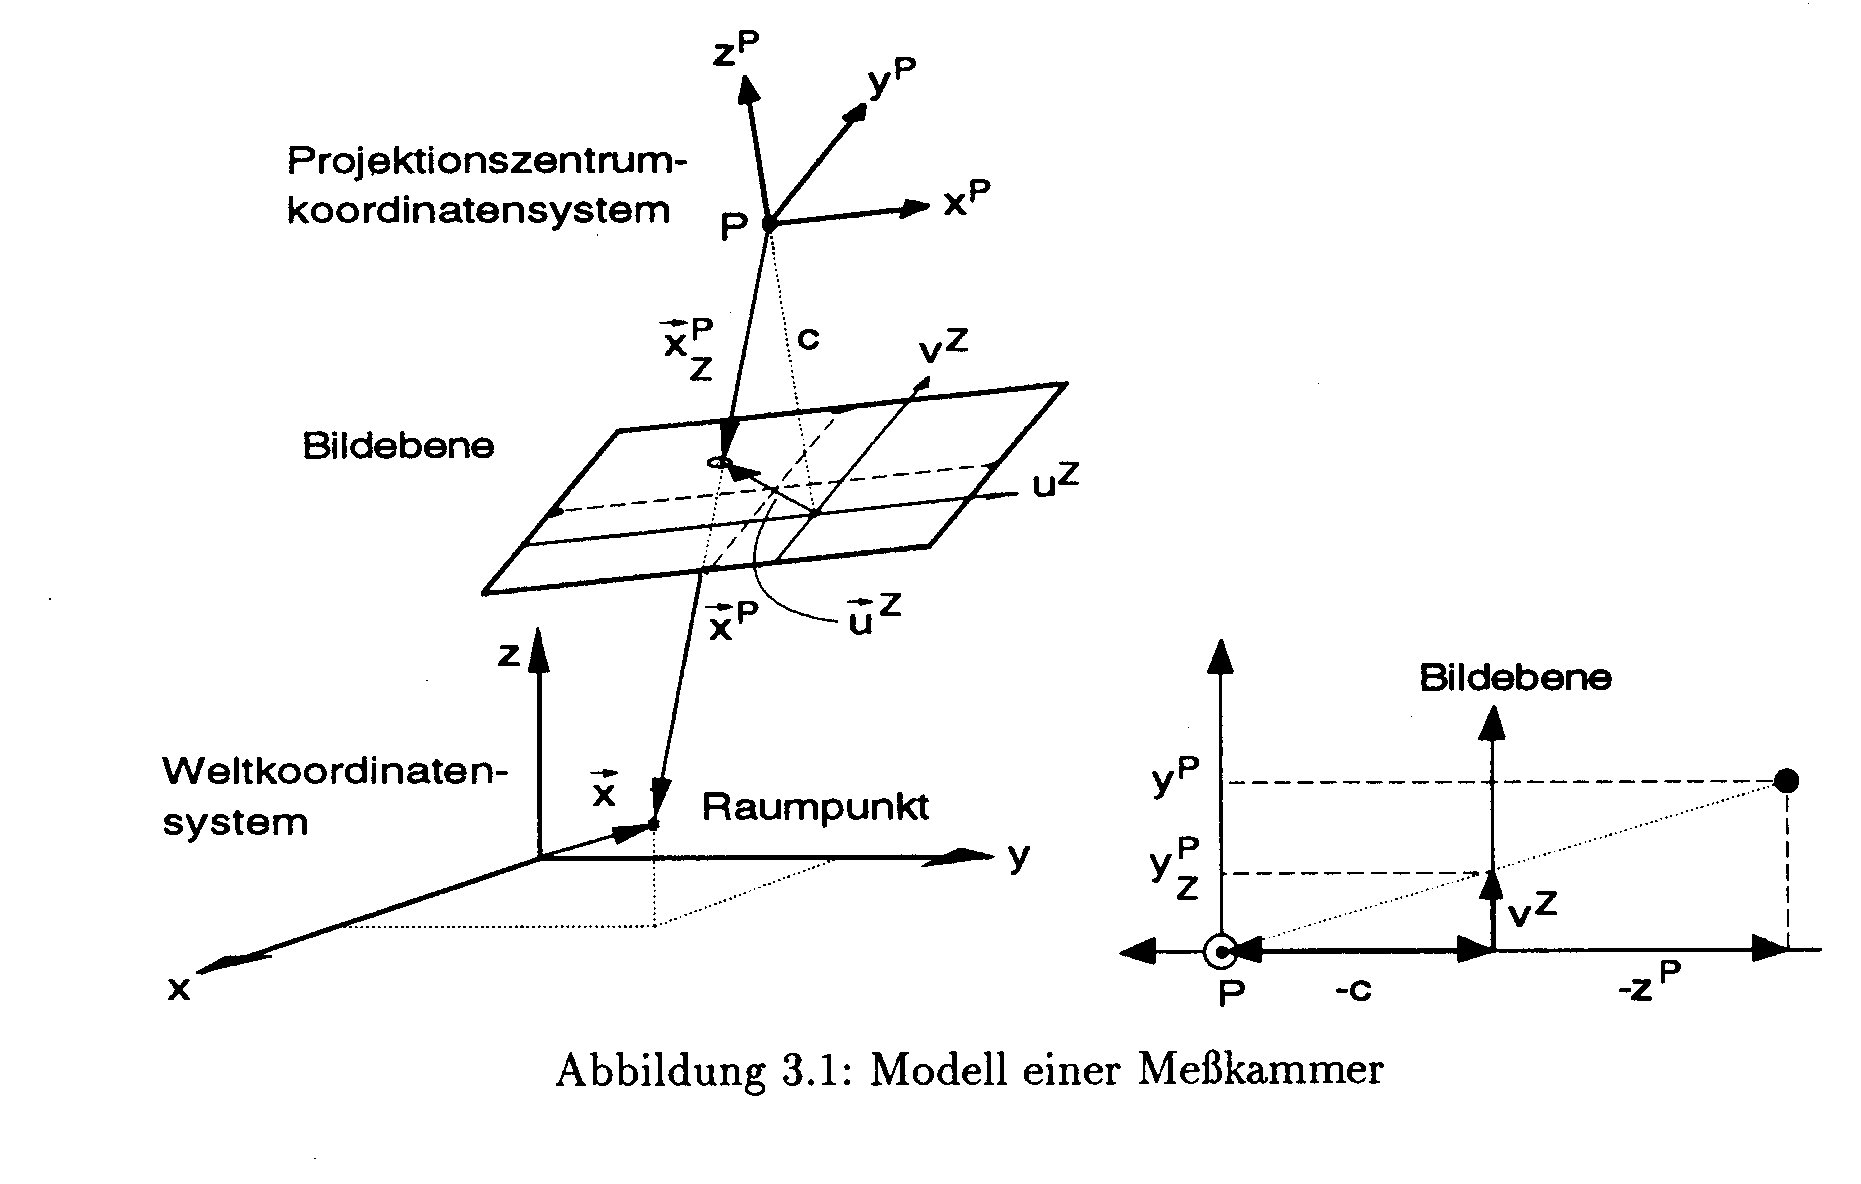
\includegraphics[width=0.65\textwidth , trim = 0mm 65mm 270mm 0mm, clip]{Bilder/cameraCalib.jpg}
			\caption{Lage des Kamerakoordinatensystems in Bezug auf Projektionsebene und Weltkoordinatensystem. \cite{Meisel:77890}}
			\label{fig:cameraCalib}
	\end{figure}

Um die verschiedenen Koordinatensysteme bei den Ausführungen in den Kapiteln \ref{sec:camCalib} und \ref{sec:planeCalib} auseinander halten zu können, wird zu Beginn eine Notation festgelegt, die in Tabelle~\ref{tab:camCalibParam} eingesehen werden kann. Zusätzlich können in der Tabelle sowohl die einzelnen Koordinatensysteme, als auch die einzelnen Berechnungsschritte der Kamerakalibrierung, sowie der Koordinatentransformation bis hinzu Unitykoordinaten, nachvollzogen werden. Lässt man die ersten zwei Zeilen der Tabelle weg, so ist eine Transformation von Weltkoordinaten $\vv{x}$ in Kamerakoordinaten $\vv{u}$ schematisch dargestellt. Dieses Schema muss für die Kamerakalibrierung von \textit{MaRC} invertiert werden und um die Koordinatentransformation in Unitykoordinaten ergänzt werden.\\

\begin{table}
	\centering
	\renewcommand{\arraystretch}{1.4}
	\begin{tabular}{|c|c|c|c|}
		\hline
		\Absatzbox{}
		& \textbf{Koordinaten} & \textbf{Komponenten}&\textbf{Transformation}\\
		\hline
		$\vv{x}^U$ & Unity &$x^U$,$y^U$,$z^U$& \\
		\cline{2-4}
		$\downarrow$ & & & Koordinatentransformation\\
		\cline{2-4}
		$\vv{x}$ & Welt &$x$,$y$,$z$&  \\
		\cline{2-4}
		$\downarrow$ & & & Koordinatentransformation\\
		\cline{2-4}
		$\vv{x}^P$ & Projektionszentrum &$x^P$,$y^P$,$z^P$& \\
		\cline{2-4}
		$\downarrow$ & & & Projektion \\
		\cline{2-4}
		$\vv{x}^P_Z$ & Projektionszentrum &$u^Z$,$v^Z$,$-c$& \\
		\cline{2-4}
		$\downarrow$ & & & Linsenverzeichnung\\
		\cline{2-4}	
		$\vv{x}^P_D$ & Verzeichnung &$u^D$,$v^D$,$-c$& \\
		\cline{2-4}
		$\downarrow$ & & & Bildebenenverkippung\\
		\cline{2-4}		
		$\vv{x}^V$ &Verkippung &$u^V$,$v^V$,$-c^V$& \\
		\cline{2-4}
		$\downarrow$ & & & Bildhauptpunktverschiebung\\
		\cline{2-4}	
		$\vv{u}$ & Sensor &$u$,$v$ & \\
		\hline
	\end{tabular}
	\caption{Parameter und Berechnungsschritte der Kamera Kalibrierung.\cite{Meisel:77890}}
	\label{tab:camCalibParam}
\end{table}


\subsubsection{Kamerakalibrierung}\label{sec:camCalib}\todo[inline, backgroundcolor=green]{Laura}
\todo[inline, color=blue]{Vera}
Es gibt viele verschiedene wissenschaftliche Ausführungen über die Durchführung einer Kamerakalibrierung, wie z.B. \cite{5982395}, \cite{888718} und \cite{faugeras1993three}. Dabei unterscheidet man häufig zwischen automatischen und manuellen Kalibrierungen. Im Folgenden wird der Algorithmus zur Kamerakalibrierung des \textit{MaRC} erläutert.  \\
Im konkreten Fall soll die uEye-Kamera (vgl. Kapitel \ref{sec:uEye}), die für Tracking-Zwecke(vgl. Kapitel \ref{sec:Tracking}) an der Decke des Entwicklungsraums befestigt ist, kalibriert werden. Dies kann, wenn gewünscht bzw. benötigt, zu Beginn der eigentlichen Anwendung durchgeführt werden. Dazu wird ein eigens für dieses Projekt angefertigter Schachbrett-Kalibrierungshelfer verwendet, der in Kapitel \ref{sec:SchachbrettKalib} beschrieben wird. Eine Beschreibung der genauen Durchführung der Kamerakalibrierung kann der ReadMe-Datei (vgl.~\ref{sec:readMe}) entnommen werden. Im Folgenden wird zunächst auf die mathematische Durchführung und dann auf die konkrete Umsetzung in Quellcode eingegangen.\\

\begin{description}
\item[Mathematische Umsetzung:] In diesem Abschnitt werden die mathematischen Grundlagen der Kamerakalibrierung erläutert. Dabei wird sowohl auf die intrinsischen, als auch auf die extrinsischen Kameraparameter eingegangen. Es wird ebenso gezeigt, die aus den Parametern eine geeignete Transformation von Kamerakoordinaten in Weltkoordinaten genildet werden kann.\\
 Wie aus Tabelle~\ref{tab:camCalibParam} hervorgeht, wird im ersten Schritt der Hauptpunkt so versetzt, dass der Koordinatenursprung des Kamerakoordinatensystems mit dem Bildkoordinatensystem übereinstimmt. Dies geschieht, indem man für die eine Achse $u^V = u - \Delta u$ und für die andere Achse entsprechend $v^V = v - \Delta v$ berechnet.\\
Zusätzlich wird die Bildebene verkippt, so dass gilt $\vv{x}^V = R_v \cdot \vv{x}^P_D$. Bezeichnet $\varphi$ den Drehwinkel um die $x^P$-Achse und $\vartheta$ den Drehwinkel um die $y^{P'}$-Achse, so lässt sich $R_v$ wie folgt berechnen:

\begin{equation}
\label{equ:Rverkippt}
R_v = 
\begin{pmatrix}
r_{v11} & r_{v12} & r_{v13} \\
r_{v21} & r_{v22} & r_{v23} \\
r_{v31} & r_{v32} & r_{v33} \\
\end{pmatrix} = 
\begin{pmatrix}
\cos\vartheta & \sin\vartheta \sin\varphi & -\sin\vartheta \cos\varphi \\
0 & \cos\varphi & \sin\varphi\\
\sin\vartheta & -\cos\vartheta \sin\varphi & \cos\vartheta \cos\varphi \\
\end{pmatrix} 
~ ~ ~ ~ ~R_v \in \mathbb{R}^{3x3}
\end{equation}

Die negative verkippte Kamerakonstante $-c^V$, die in Tabelle~\ref{tab:camCalibParam} aufgeführt ist, berechnet sich wie in~\citep{Meisel:77890} beschrieben nach der Formel:

\begin{equation}
-c^V = - \frac{c+u^V \cdot r_{v13} + v^V \cdot r_{v23}}{r_{v33}}
\end{equation}

Im zweiten Schritt wird im Allgemeinem die Linsenverzeichnung herausgerechnet. Im vorliegenden Fall wurde bewusst auf diesen Schritt verzichtet und die zugehörigen Entzerrungskoeffizienten werden für alle weiteren Berechnungen auf null gesetzt. Dieses Vorgehen wurde gewählt, da einige Tests gezeigt haben, dass die berechneten Entzerrungskoeffizienten stark voneinander abgewichen sind, obwohl dies beim Benutzen der gleichen Kameraeinstellungen und dem gleichen Objektiv nicht der Fall sein dürfte.\\
Weil wie bereits beschrieben, die Linsenverzeichnung vernachlässigt wurde, kann man Schritt 1 und 2 zu einem Schritt zusammenfassen und vereinfacht darstellen. Dieser erste Schritt, also die Hauptpunktverschiebung und Bildebenenverkippung, lässt sich mit Hilfe der intrinsischen Kameramatrix $M_{intrinsisch}$ zusammenfassen. Diese beinhaltet neben den Brennweiten $f_u$ und $f_v$ noch die Koordinaten des Hauptpunktes $u^V$ und $v^V$ in Bildkoordinaten und hat somit vier Freiheitsgrade.

\begin{equation}
\label{equ:intrinsic}
M_{intrinsisch} = 
\begin{pmatrix}
f_u & 0 & 0 & u^V \\
0 & f_v & 0 & v^V\\
0 & 0 & 1 & 0 \\
\end{pmatrix} 
~ ~ ~ ~ ~M_{intrinsisch} \in \mathbb{R}^{3x4}
\end{equation}

Während eine dreidimensionale Rotation im Allgemeinen mit Matrix $R$ aus Formel~\ref{equ:Rotation} beschrieben werden kann, reicht für die Translation ein Vektor, wie $t$ aus Formel~\ref{equ:Translation} aus.\

\begin{equation}
\label{equ:Rotation}
R= R_\gamma ~R_\beta ~R_\alpha =
\begin{pmatrix}
r_{11} & r_{12} & r_{13} \\
r_{21} & r_{22} & r_{23} \\
r_{31} & r_{32} & r_{33} \\
\end{pmatrix}
~ ~ ~ ~ ~R \in \mathbb{R}^{3x3}
\end{equation}

\begin{equation}
\label{equ:Translation}
t=
\begin{pmatrix}
t_x & t_y & t_z
\end{pmatrix}^T
~ ~ ~ ~ ~t \in \mathbb{R}^{3x1} 
\end{equation}

Diese beiden Transformationen können wie in Formel~\ref{equ:extrinsic} zur extrinsischen Kameramatrix $M_{etrinsisch}$ zusammengefasst werden. Diese hat sechs Freiheitsgrade, nämlich drei für den Translationsvektor $t$ und drei für die Eulerwinkel der Rotationsmatrix $R$ für die dementsprechend gelten muss $R \in SO(3)$.

\begin{equation}
\label{equ:extrinsic}
M_{extrinsisch}= 
\begin{pmatrix}
R &|& t \\
\end{pmatrix} 
~ ~ ~ ~ ~M_{extrinsisch} \in \mathbb{R}^{3x4}
\end{equation}

Schritt 1 und 2 lassen sich vereinfachen, indem man die intrinsische Kameramatrix $M_{intrinsisch}$ und die extrinsische Kameramatrix $M_{extrinisch}$ nach der Formel~\ref{equ:inAndEx} zu einer Matrix $M$ zusammenfasst.

\begin{equation}
\label{equ:inAndEx}
M = M_{intrinsisch} \cdot M_{extrinsisch}~ ~ ~ ~ ~M\in \mathbb{R}^{3x4}
\end{equation}

Die Umrechnung von Kamerakoordinaten in Weltkoordinaten kann dann mit der invertierten Matrix $M$, wie in Formel~\ref{equ:SensInWorld} berechnet werden. \

\begin{equation}
\label{equ:SensInWorld}
\vv{x} = M^{-1} \cdot \vv{u}
\end{equation}

An diesem Punkt hat man die Kamerakoordinaten vollständig in Weltkoordinaten überführt und sucht nun eine Transformationsmatrix um diese Punkte auf ihre korrespondierenden Punkte (vgl. Kapitel \ref{sec:Korrespondenz}) in Unitykoordinaten abzubilden. Die dazu benötigte affine 3D-Transformation wird in Kapitel \ref{sec:planeCalib} erläutert.
\end{description}

Zu diesem Zeitpunkt sollte nun das Kamerakoordinatensystem mit dem Weltkoordinatensystem übereinstimmen und es kann sich im nächsten Schritt darum gekümmert werden, dass das Kamerakoordinatensystem verschoben und gedreht wird. Dieser Schritt und alle weiteren Schritte, die im Zusammenhang mit der Transformation von Kamerakoordinaten in Weltkoordinaten bzw. Weltkoordinaten in Unitykoordinaten stehen, werden in Kapitel~\ref{sec:planeCalib} erläutert. Hierbei sei noch einmal angemerkt, dass eine Kamerakalibrierung nur mit anschließender Kalibrierung des Arbeitsbereiches durchgeführt werden kann.


\subsubsection{Kalibrierung des Arbeitsbereichs}\label{sec:planeCalib} \todo[inline, color=green]{Laura}
\todo[inline, color=blue]{Vera}
Wie bereits beschrieben, kann eine Kalibrierung des Arbeitsbereichs entweder mit vorheriger Kamerakalibrierung oder einzeln durchgeführt werden. In letzterem Fall wird dann die zuletzt verwendete Kamerakalibrierung geladen (vgl. Abschnitt \ref{sec:saveCalib}. Die Durchführung der Kalibrierung wird in der ReadMe-Datei (vgl.~\ref{sec:readMe}) erläutert. Grob gesagt, werden über Knopfdruck am Kalibrierungscontroller (vgl. Abbildung~\ref{fig:KontrollerMarc}) 25 seiner Positionen sowohl in Kamerakoordinaten, als auch in Unitykoordinaten gespeichert. Man erhält also 25 korrespondierende Punktepaare (vgl. Kapitel \ref{sec:Korrespondenz}).\\
Allgemein betrachtet hat die Arbeitsbereichskalibrierung zwei verschiedene Aufgaben: Zum einen wird hierbei ein Bereich festgelegt, indem die Objekte getrackt werden und zum anderen wird mittels der verschiedenen Positionen der Kalibrierungspunkte, die affine Transformationsmatrix bestimmt, die im weiteren Verlauf als Umrechnung zwischen Kamerakoordinaten und Unitykoordinaten fungiert. Beide Teilbereiche werden in den Absätzen \grqq Begrenzung des Arbeitsbereichs\grqq ~bzw. \grqq Affine Transformation\grqq ~weitergehend erläutert.

\begin{figure}
	\centering
	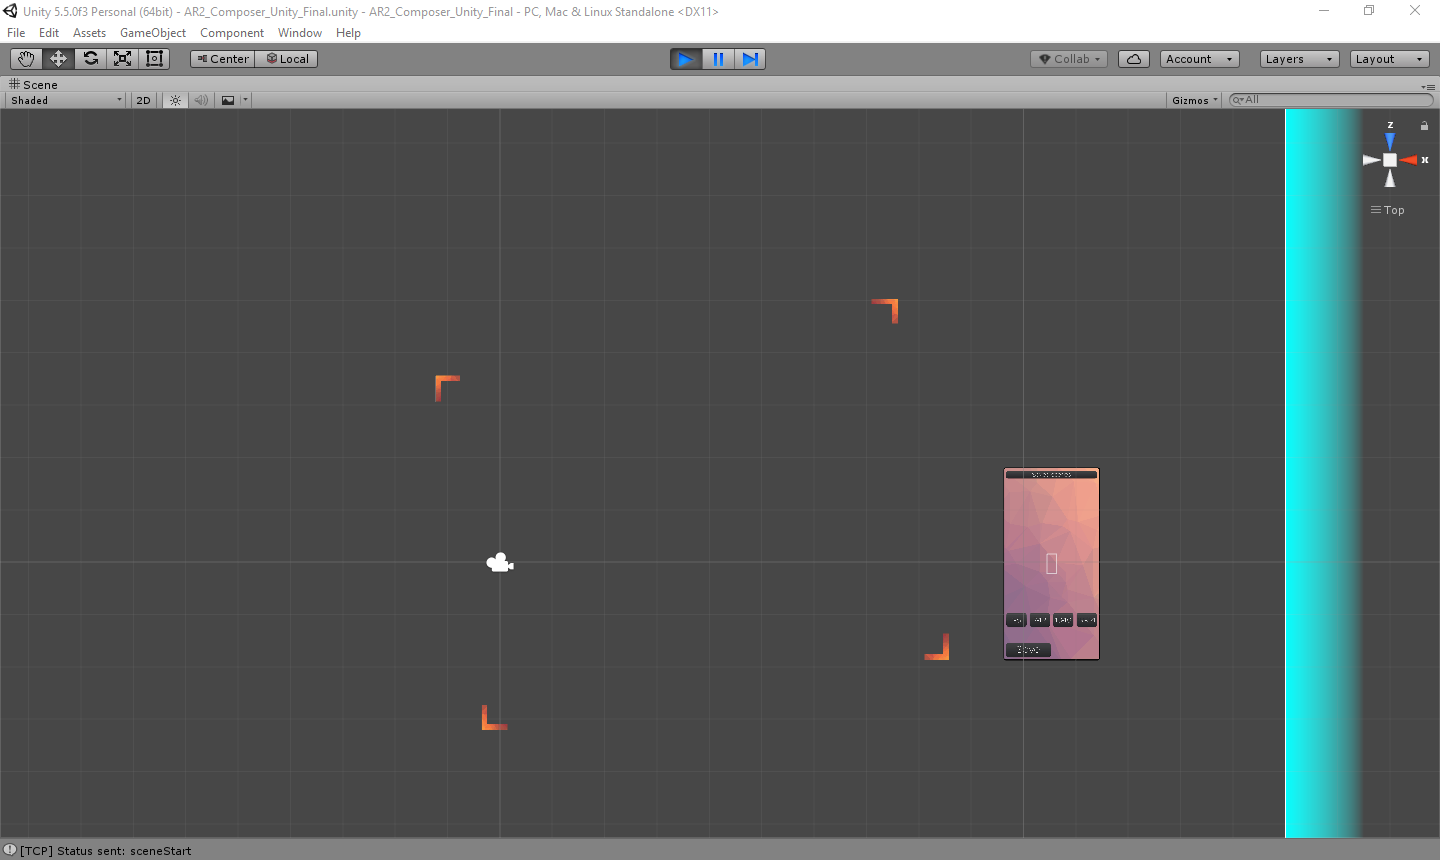
\includegraphics[width=\textwidth, trim=7cm 2cm 5cm 6cm, clip]{Bilder/Neue Screenshots/Arbeitsbereich.PNG}
	\caption{Begrenzung des Arbeitsbereichs in der \emph{Unity}-Simulation.}
	\label{fig:begrenzungArbeitsbereich}
\end{figure}

\begin{description}
\item[Begrenzung des Arbeitsbereichs] Die ersten vier Punktepaare dienen dazu den Arbeitsbereich zu definieren. Sie müssen in einer klar definierten Reihenfolge, nämlich im Uhrzeigersinn und in der linken unteren Ecke beginnend, durchgeführt werden. Dabei wird bei beiden Systemen (Tracking-Anwendung und \emph{Unity}-Simulation) unterschiedlich vorgegangen, was zu leicht abweichenden Arbeitsbereichen führen kann. Es wird ausdrücklich empfohlen sich dabei an den Tischkanten zu orientiert und beispielsweise die Kante der Auflage des Kalibrierungscontrollers (vgl. Kapitel \ref{sec:calibController}) daran auszurichtet und somit eine ungefähr rechteckförmige Fläche aufzuspannen. \\
Für die Tracking-Anwendung reicht es aus, den 1. und 3. Punkt zu nehmen und damit ein Rechteck aufzuspannen. Dies geschieht in der \texttt{compute\-Plane\-Cali\-bration()}-Methode in der \texttt{Plane\-And\-Affine\-Calibration.cpp}-Klasse. Der so definierte Arbeitsbereich dient hier vor allem dazu, zu entscheiden, ob ein Marker noch im Anwendungsbereich ist und somit fortlaufend getrackt werden muss, oder ob er diesen Bereich verlassen hat und seine ID, sowie alle anderen Eigenschaften zurückgesetzt werden müssen (vgl. Kapitel \ref{sec:MarkerDetektion}). In Abbildung \ref{fig:DebugScreenshot} ist der so aufgespannte Arbeitsbereich in rot dargestellt.\\
Auf \emph{Unity}-Seite werden die gesamten ersten vier Punkte genutzt um den Arbeitsbereich festzulegen. Dies hat den Grund, dass der Arbeitsbereich bei der Simulation an allen vier Ecken durch kleine "`Winkel"', wie in Abbildung~\ref{fig:begrenzungArbeitsbereich} dargestellt, begrenzt wird. Zunächst war der Arbeitsbereich in der \emph{Unity}-Simulation ebenfalls nur durch zwei Punkte definiert, sodass der Bereich immer ein Rechteck auf dem Tisch darstellte. Es stellte sich jedoch heraus, dass ein im Kamerabild auf Tracking-Seite definiertes Rechteck übertragen auf die \emph{Unity}-Simulation nicht hinreichend genau als Rechteck auf dem Tisch abgebildet wurde. Dies führte dazu, dass Marker, die in der Simulationsanwendung noch innerhalb des Spielfelds zu sein schienen, auf Tracking-Seite bereits deregistriert worden waren, oder umgekehrt. Um dieses Abbildungsproblem zu umgehen, wurden anschließend vier Punkte für die Definition des Arbeitsbereichs in der \emph{Unity}-Simulation verwendet. Der Nachteil hierbei ist, dass der Arbeitsbereich bei genauem Hinsehen nicht genau einem Rechteck entspricht, sondern eher einem Parallelogramm.

\item[Affine Transformation] Die restlichen 21 Controller-Positionen werden genutzt, um eine affine Transformation von Weltkoordinaten in Unitykoordinaten zu finden. An dieser Stelle kann davon ausgegangen werden, dass die Mittelpunkte der \textit{ArUco} Marker über die in Kapitel \ref{sec:camCalib} beschriebene Transformation bereits in Weltkoordinaten vorliegen. Dabei werden die Position nicht wie bei der Begrenzung des Arbeitsbereichs für beide Systeme (Tracking und Unity) getrennt verarbeitet, sondern sie werden als korrespondierende Punkte (vgl. Kapitel \ref{sec:Korrespondenz}) verstanden. Mit anderen Worten, soll in diesem Schritt des Algorithmus jeder dieser 21 Punkte in Weltkoordinaten, möglichst fehlerfrei auf sein entsprechendes Pendant in Unitykoordinaten projiziert werden. \\
Es gilt also die in Gleichung \ref{equ:affin} der Vollständigkeit halber aufgeführte Matrix zu bestimmen. Da es geeignete Werte für $a, b, c$ und $d$, sowie die Translationsparameter $t_x$ und $t_y$ zu finden gilt, hat die gesuchte Transformation 6 Freiheitsgrade. Zur Abschätzung der bestmöglichen Matrix $M_{affin}$ eignet sich vor allem der RANSAC-Algorithmus ~\cite{articel:RANSAC}. Dieser wird ebenso für die in diesem Projekt verwendete \textit{OpenCV}-Methode \texttt{estimateAffine3D()} verwendet. Dieser Methode können alle 21 korrespondierenden Punktepaare übergeben werden. 

\begin{equation}
\label{equ:affin}
M_{affin} = 
\begin{pmatrix}
a & b & t_x \\
c & d & t_y \\
0 & 0 & 1  \\
\end{pmatrix} 
~ ~ ~ ~ ~M_{affin} \in \mathbb{R}^{3x3}
\end{equation}
\end{description}

\subsubsection{Kalibrierungsfehler} \label{sec:calibError}\todo[inline, color=green]{Laura}
\todo[inline, color=blue]{Vera}
In den Kapiteln~\ref{sec:camCalib} und~\ref{sec:planeCalib} wird der Algorithmus zur Berechnung der Koordinatentransformation von Kamerakoordinaten in Unitykoordinaten beschrieben. Beim Benutzen des fertig kalibrierten System fällt jedoch auf, dass die Aluminiumwürfel nicht immer deckungsgleich mit ihrem gerenderten Pendant sind. Der beobachtete Fehler variiert bei jeder Kalibrierung. In Abbildung~ref{fig:markierterFehler} wird ein Kalibrierungsfehler in vertretbarer Größenordnung gezeigt. Dieser ist mit weiß markiert. Im Idealfall würden die beiden weißen Kreise deckungsgleich sein. Wird ein deutlich größerer Fehler beobachtet, so ist es sinnvoll neu zu kalibrieren. Im Folgenden werden mögliche Gründe für die Positionsabweichung von dem Würfel-Marker und seinem virtuellen Marker diskutiert. \\
Neben der Rechenungenauigkeit und Rundungsfehlern, die sich über die diversen Rechenschritte (vgl. Abschnitt~\ref{sec:camCalib} und ~\ref{sec:planeCalib}) hinweg aufaddieren, sollen in diesem Kapitel systembedingte mögliche Fehlerquellen aufgeführt werden. Man kann davon ausgehen, dass sich der Fehler großteils durch Fehlerfortpflanzung \cite{schmalstieg2016augmented} ergibt.\\ 
Aufgrund der Auflösung der für das Tracking genutzten \textit{IDS uEye}-Kamera (vgl. Abschnitt \ref{sec:uEye}) ist die Genauigkeit des Trackings begrenzt und die Positionen der Würfel-Marker können nicht beliebig genau ermittelt werden. Dieser Effekt wird durch Einflüsse wie z.B. Bildrauschen weiter verstärkt. Es ist also davon auszugehen, dass die Mittelpunkte der verfolgten Marker, die als ein Part in die korrespondierenden Punktepaare (vgl. Abschnitt~\ref{sec:Korrespondenz}) eingehen, schon einen gewissen Fehler aufweisen. \\
Da mittels des RANSAC-Algorithmus~\cite{articel:RANSAC} lediglich eine Schätzung ermittelt wird, ist die affine Transformationsmatrix $M_{affin}$ nicht gänzlich fehlerfrei. \\
Zusätzliche Fehler bei der Registrierung können durch Latenz entstehen. Nämlich immer dann, wenn eine Zeitdifferenz zwischen der Messung der Position in Kamerakoordinaten und der eigentlichen Darstellung nach entsprechender
Verarbeitung entsteht. Solche Systemverzögerungen werden allerdings nur bei Bewegungen sichtbar und sind deshalb für die beobachteten Fehler bei ruhendem Aluminiumwürfel nicht als mögliche Fehlerquelle auszumachen. 

\begin{figure}
	\centering
	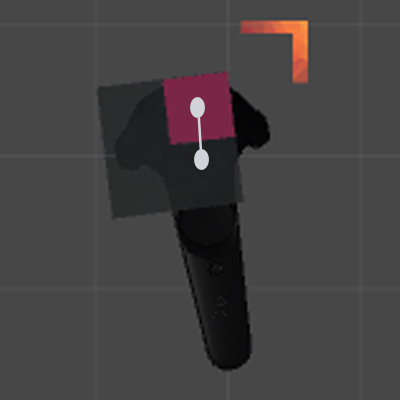
\includegraphics[scale=0.6]{Bilder/Neue Screenshots/Kalibrierungsfehler_OR-KLEIN.jpg}
	\caption{Mit weiß markierter möglicher Kalibrierungsfehler.}
	\label{fig:markierterFehler}
\end{figure}



\subsubsection{Schnittstelle der beiden Kalibrierung} \label{sec:CalibSteuerung}\todo[inline, backgroundcolor=green]{Laura und Vera}
\todo[inline, color=red]{Laura}
Wie bereits erwähnt, dient die \texttt{Calibration.cpp}-Klasse als Schnittstelle für die Kamerakalibrierung (vgl. Abschnitt~\ref{sec:camCalib}) und die Arbeitsbereichskalibrierung (vgl. Abschnitt~\ref{sec:planeCalib}). Diese Schnittstelle stellt alle erforderlichen Funktionen für beide Kalibrierungen und die benötigten Zugriffe auf die generierten Daten zur Verfügung. 

Die \texttt{runPoseEstimation()}-Methode ist zuständig für die Generierung der Kameramatrix \texttt{camMatrix}  ($M_{intrinsisch}$ aus Gleichung \ref{equ:intrinsic})  und die Koeffizienten zur Behebung der Linsenverzeichnung \texttt{distCoeffs}. Beide werden mit dem Modul \texttt{calib3D} der \textit{OpenCV} Bibliothek in der Klasse \texttt{calib\-With\-Chess\-board.cpp} berechnet und anschließend in der Methode \texttt{generate\-Cam\-Mat\-And\-Dist\-Mat()} der Klasse \texttt{Pose\-Esti\-mation.cpp} für die spätere  Verwendung gespeichert. \\
Die Klasse \texttt{calib\-With\-Chess\-board.cpp} implementiert den modifizierten Beispielcode \texttt{calibration.cpp} \cite{website:calibexample} aus dem \textit{GitHub} Repository der \textit{OpenCV} Bibliothek. Die Modifikation ermöglicht die Kompatibilität mit dem restlichen Programm. Vor dem Speichern und der Weiterverbreitung werden die \texttt{disCoeffs} auf null gesetzt, da die Entzerrung des Bildes nicht zuverlässig ist. Die explizite Bestimmung der intrinsischen und extrinsischen Matrizen findet in der \textit{OpenCV}-Methode \texttt{calibrate\-Camera()} auf Grundlage von mehreren Aufnahmen eines fest definierten Kalibrierungsmusters (vgl. Abschnitt~\ref{sec:SchachbrettKalib}) statt.

Wie in Kapitel \ref{sec:planeCalib} erklärt werden mittels der Arbeitsbereichskalibrierung zwei doch recht unterschiedliche Ziele verfolgt. Zum einen wird der tatsächliche Arbeitsbereich festgelegt und zum anderen wird die affine Transformation von Weltkoordinaten in Unitykoordinaten berechnet. Beide Aufgaben werden in der Schnittstelle mit der Funktion \texttt{generate\-Affine\-And\-Plane\-Calib()} aufgerufen, welche die entstprechenden Implementierungen in der Klasse \texttt{PlaneAndAffineCalibration.cpp} ansteuert und die Ergebnisse in Textfiles abspeichert. Die Methoden \texttt{load\-Affine\-Transform()} und \texttt{load\-Image\-Plane()} laden bei keiner neuen Kalibrierung, die zuletzt abgespeicherten Daten (vgl. Abschnitt \ref{sec:saveCalib}). \\

Die affine Transformation wird auf Grundlage der korrespondierenden Punktepaare (vgl. Abschnitt \ref{sec:Korrespondenz}) berechnet. Hierzu wird in der Methode \texttt{compute\-Affine\-Trans\-formation()} die Funktion \texttt{estimate\-Affine\-3D()} der \textit{OpenCV} Bibliliothek aufgerufen, welche die affine Transformationsmatrix mit Hilfe des RANSAC-Algorithmus abschätzt~\cite{articel:RANSAC}.
>>>>>>> 0b0f17e7968ff0269eb005bca8a9908d2a753f06

\subsubsection{Speichern und Laden der Kalibrierungen}\label{sec:saveCalib}\todo[inline, color=green]{Laura}
\todo[inline, color=blue]{Vera}
Sowohl die Kamerakalibrierung als auch die Arbeitsbereichskalibrierung werden automatisch nach der Erstellung abgespeichert. Das gibt dem Benutzer beim nächsten Ausführen des System die Möglichkeit, folgenden 3 Möglichkeiten: 
\begin{description}
	\item[1. Beide Kalibrierungen durchführen]: In diesem Fall wird zunächst eine Kamerakalibrierung durchgeführt, wie sie in Kapitel ~\ref{sec:camCalib} beschrieben ist und anschließend wird eine Kalibrierung des Arbeitsbereiches (vgl. Kapitel ~\ref{sec:planeCalib}) vorgenommen. Alle daraus resultierenden Kamerakalibrierungs-Parameter werden mittels der \texttt{saveCameraParams()}-Methode (vgl. \texttt{PoseEstimation.cpp}-Klasse) gespeichert. Die notwendigen Eckpunkte des Arbeitsbereichs werden direkt nach ihrer Erstellung über die \texttt{computePlaneCalibration()}-Methode abgespeichert und die affine Transformation wird über die \texttt{saveAffineTransform()}-Methode (vgl. \texttt{PlaneAndAffineCalibration.cpp}-Klasse) in ein Textfile gesichert. Somit stehen alle benötigten Parameter - wenn gewünscht - für den nächsten Systemstart bereit.
	
	\item[2. Nur die Arbeitsbereichskalibrierung durchführen]: Entscheidet sich der Benutzer dafür, dass eine Kamerakalibrierung nicht notwendig ist, so können die entsprechenden Parameter über die \texttt{loadCameraMat()}-Methode aus der \texttt{PoseEstimation.cpp}-Klasse geladen werden. Der Arbeitsbereich kann dann wie in Kapitel ~\ref{sec:planeCalib} beschrieben kalibriert werden und die neue Kalibrierung wird wie unter 1. beschrieben abgespeichert. Die alte Kamerakalibrierung wird allerdings beibehalten und muss nicht erneut gesichert werden. 
	
	\item[3. Keine Kalibrierungen durchführen]: Wenn der Nutzer unter den gleichen Bedingungen, wie bei der letzten Systemverwendung weiterarbeiten möchte, ist es sinnvoll die komplette Kalibrierung zu laden. Für die Kamerakalibrierung geht man dabei wie unter 2. beschrieben vor. Für das Laden der Arbeitsbereichskalibrierung stehen hierfür die Methoden \texttt{loadImagePlane()} und \texttt{loadAffineTransform()} aus der \texttt{PlaneAndAffineCalibration.cpp}-Klasse zur Verfügung.
\end{description}
\subsection{Marker Detektion}\label{sec:MarkerDetektion} \todo[inline, color = green]{Vera}
\todo[inline, color=red]{Laura}
Nach Abschluss der erfolgreichen Kalibrierung bzw. des Ladens einer gespeicherten Kalibrierung (vgl. Abschnitt \ref{sec:saveCalib}) beginnt das Tracking Programm, sowohl damit die \textit{ArUco} Marker, als auch die leuchtend grünen Rechtecke zu detektieren. Die codebasierten \textit{ArUco} Marker ermöglichen es den Marker nach längerer Verdeckung wieder eindeutig seiner entsprechenden Registrierungs-ID (RID) zu zuordnen. Somit wird Fehlzuordnungen oder sprunghaften Vertauschungen von benachbarten Würfel Markern vorgebeugt. Alle Methoden zur Detektierung der beiden Markertypen werden von der Klasse \texttt{MarkerDetection.cpp} zur Verfügung gestellt und mit der Funktion \texttt{run\-Marker\-Detection()} aufgerufen. \\
Die detektierten Marker werden nur verfolgt wenn sie innerhalb eines festgelegten Arbeitsbereichs positioniert sind. Zur Registrierung eines Marker-Objektes (vgl. Abschnitt~ \ref{sec:MarkerObjekte}) muss der Würfel-Marker in den anzeigte Arbeitsbereich geschoben werden und zur Abmeldung wieder heraus. Demzufolge werden Würfel-Marker deren \textit{ArUco}-ID (AID) noch unbekannt ist registriert und Würfel-Marker, welche den Arbeitsbereich verlassen, zurückgesetzt und die RID wieder freigeben. Der Arbeitsbereich wird während der Kalibrierung des Arbeitsbereichs (vgl. Abschnitt~\ref{sec:planeCalib}) definiert, indem der erste und dritte Schwerpunkt der detektierten \textit{ArUco} Marker das Rechteck des Feldes aufspannen. \textcolor{red}{Das mit dem Schwerpunkt verstehe ich nicht. Ist damit der Schwerpunkt eines AruCoMarkers gemeint? Wenn ja würde ich den Satz umstellen, sodass man das direkt checkt}\\
Zunächst werden während der Marker Detektion die grünen Rechtecke mit Hilfe eines simplen \textit{Greenkeying} erfasst und im Anschluss die erforderlichen \textit{ArUco} Marker der Würfel Marker. Letztere können bekannterweise unter Umständen nur im ruhenden Status erfasst werden, da eine mögliche Bewegungsunschärfe bei schnellen Verschiebungen (vgl. Abschnitt~\ref{sec:MarkerTracking}) eine korrekte Erfassung nahezu unmöglich macht. 
Aus diesem Grund werden neben den codebasierten Muster auch die leuchtend grünen Rechtecke verfolgt um einen Würfel-Marker auch bei schnelleren Bewegungen zu verfolgen.
\subsubsection{Detektion der grünen Rechtecke}\label{sec:GreenRects}\todo[inline, color=green]{Vera}
\todo[inline, color=red]{Laura}
Das Ziel dieses Verfahren ist es eine \textit{Oriented Bounding Box}(OBB) von jedem erkannten grünen Rechteck zu erstellen. Die OBB beinhalten Informationen über die Größe, den Schwerpunkt, die vier Eckpunkte sowie den Rotationswinkel im Verhältnis zum Bildkoordinatensystem. Alle genannten Informationen werden in einem \texttt{RotatedRect} gespeichert, welches eine Objektklasse der \textit{OpenCV} Bibliothek ist.\\
Bei der Detektion der grünen Rechtecke müssen diese zunächst mit Hilfe einer Binarisierung segmentiert werden. Jedoch ist die Aufnahme zu diesem Zeitpunkt ein Bild mit RGB Farbmodus, dessen Grundfarben von der Helligkeit abhängig sind. Somit müssten, je nach Beleuchtungsverhältnisse, die Schwellwerte einer Binarisierung geeignet angepasst werden. Im Gegensatz zum RGB Farbraum ist der HSI Farbraum unabhängig von der Beleuchtung, da er seine Grundbestandteile aus den Werten von Farbton (H), Sättigung (S) und Helligkeit (I) definiert. Folgerichtig ist es theoretisch ausreichend nur den Farbton zu beachten um Objekte oder Teilbereiche einer bestimmten Farbe zu segmentieren.\textcolor{red}{Gute Erklärung von RGB und HSI. Kannst du das noch so umschreiben, dass hervorgeht das der HSI Farbraum nicht nur besser wäre, sondern das du tatsächliche eine transformation von RGB nach HSI gemacht hast. Dann versteht man glaube ich die nächste Passage besser}\\
Die Binarisierung jedes Pixel $x \in (\Re^3 | 0 \ge x_H \le 255, 0 \ge x_S \le 255, 0 \ge x_I \le 255$) \textcolor{red}{Meinst du hier vielleicht $\mathbb{R}^{3}$ anstatt $\Re^3$}erfolgt unter den Bedingungen aus Gleichung \ref{equ:Threshold}, welche alle nicht grünen Bildsektionen schwarz maskiert und nur die grünen Bildbereiche weiß. An dieser Stelle wurden neben dem Farbton auch die Sättigung und Helligkeit betrachtet. Durch die Eingrenzung der Sättigung wird sichergestellt, dass nur grüne Bereiche mit einer hohen Leuchtkraft berücksichtigt werden. Während die leichte Einschränkung der Helligkeit das Rauschen im Schwarz-Weiß-Bild verringert. Das verbleibende Bildrauschen wird durch einen Median Rangordnungsfilter mit einer Kernelgröße von $5\times5$ eliminiert. Diese beide Methoden sind Teil der \textit{OpenCV} Bibliothek. \textcolor{red}{Für den letzten Satz würde ich schreiben: Sowohl die Binarisierung, als auch der Rangordnungsfilter können mit Methoden aus der  \textit{OpenCV} Bibliothek umgesetzt werden.}

\begin{equation}
\label{equ:Threshold}
I(x) = \begin{cases}
255 & wenn \ 65 \ge x_H \le 85, \ 120 \ge x_S \le 255, \ 22 \ge x_I \le 255\\\
0 & sonst
\end{cases}
\end{equation}

Im binarisierten Bild werden im Anschluss zur Detektierung der OBB die Rechteckkanten mit einem Canny Kanten Detektor extrahiert~\cite{article:Canny}. Im \textcolor{red}{daraus??} resultierenden Kantenbild werden mit Hilfe eines Kantenverfolgungsalgorithmus \cite{article:FindConturs} die Konturen generiert. Dieser Algorithmus erstellt eine hierarchische Sammlung von allen Punkten der äußersten Konturen eines Objektes. Aus dieser Sammlung wird die OBB mit dem \textit{Douglas Ramer Peucker} Algorithmus \cite{article:RamerPeucker} approximiert. Während der Approximation werden die Konturen geglättet und somit an ein ideales Rechteck angenähert. In Abbildung \ref{fig:DebugScreenshot} ist sind die generierten OBB weiß dargestellt und es ist deutlich zusehen, dass die Annäherung sehr genau ist.
\begin{figure}[H]
	\centering
	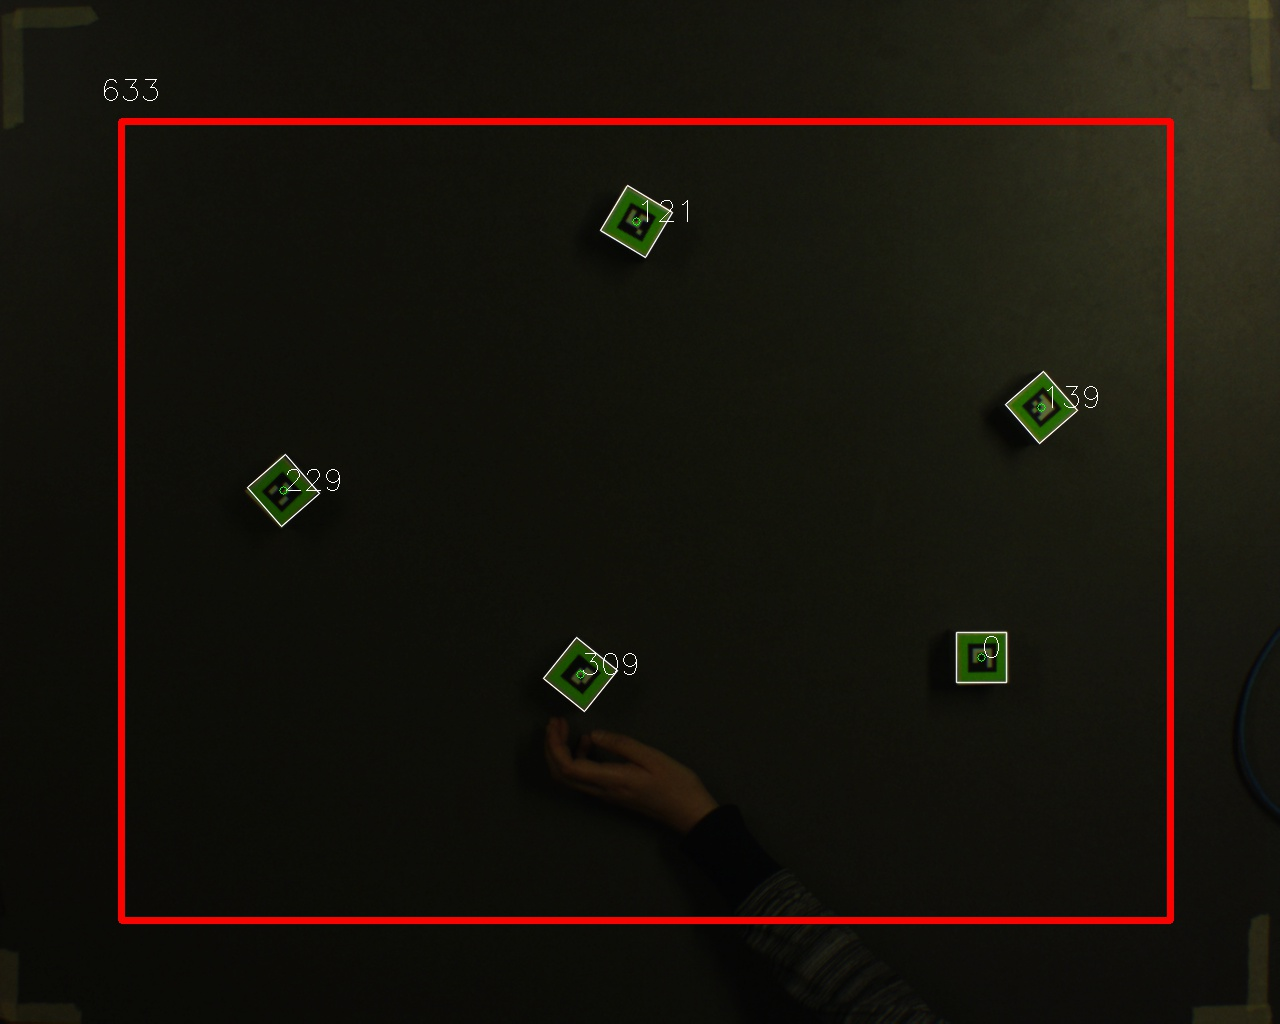
\includegraphics[width=3in]{Bilder/TrackingScreenshot_x.jpg}
	\caption{Screenshot des Tracking Programms. Die weißen Konturen sind die detektierten grünen Rechtecke. Alle Beschriftungen der Marker zeigen die resultierenden Winkel an und der äußere rote Rahmen stellt den kalibrierten Arbeitsbereich dar.}

	\label{fig:DebugScreenshot}
\end{figure}
\subsubsection{ArUco Marker Detektion}\label{sec:ArucoMarkerTracking}\todo[inline, color=green]{Vera}
\todo[inline, color=red]{Laura}
 In der Klasse \texttt{MarkerDetection.cpp} werden in der Funktion \texttt{detect\-Aruco\-Marker()} alle \textit{ArUco} Marker detektiert \cite{article:Aruco2014}, die sich im Bild befinden. Die gesamte Detektion wird durch die Methode \texttt{detect\-Markers()} der \textit{ArUco} Bibliothek aufgerufen und als Ergebnis bekommt jeweils die vier Eckpunkte der erkannten Marker Muster. In dieser Methode werden die drei benötigten Schritte zur Detektion der Marker implementiert. Zunächst wird das Graustufenbild mit adaptiven lokalen Schwellwerten binarisiert und anschließend die Kanten des binären Bildes mit einem Canny Filter \cite{article:Canny} herausgefiltert. Von diesen Objektkanten werden, wie bei den OBBs (vgl. Abschnitt \ref{sec:GreenRects}), die Konturen extrahiert und vervollständigt.
  
 Der letzte Schritt sieht sowohl die Positionsabschätzung als auch die Verfeinerung der erkannten Markerpunkte vor. Zur Verbesserung der detektierten Punkte kann eine Verfeinerung der Positionen mit einer linearen Regression erreicht werden. Anschließend kann mit den generierten Konturpunkten die AID ermittelt werden, indem die Werte mit den Daten aus dem ausgewählten Dictionary abgeglichen wird.

 Die Positionsabschätzung dient dazu die Markerposition mit Hilfe des Levenberg-Marquardt Algorithmus \cite{article:Levenberg} im Kameraraum zu bestimmen. Für diesen Prozess stellt die \textit{ArUco} Bibliothek die Methode \texttt{esti\-mate\-Pose\-Single\-Markers()} zur Verfügung, welche für eine erfolgreiche Schätzung mehrere Parameter verlangt. Zum einen werden die vier äußeren Eckpunkte des Codemusters benötigt und zum anderen die reale Kantenlänge eines Markers von $0.04$m. Weiterführend, werden auch die intrinsische und extrinschen Kameramatrizen benötigt, welche während der letzten Kamerakalibrierung (vgl. Abschnitt \ref{sec:camCalib}) erstellt wurden.

 
\subsection{Marker Objekt Definition}\label{sec:MarkerObjekte}\todo[inline, color=green]{Vera}
\todo[inline, color=red]{Laura}
Die Marker Objekte der Klasse \texttt{Marker.cpp} speichern alle benötigten Parameter und Informationen der registrierten Würfel-Marker. Zu diesen Daten gehören unter anderem die RID \texttt{id}, die aktuelle AID \texttt{arucoID} des zugeteilten Würfel Markers sowie die entsprechende OBB \texttt{rect} des letzten Frames. \textcolor{red}{Würde das hervorgehobene evtl. in Klammern schreiben} Weitere boolesche Variablen wie \texttt{isVis} und \texttt{isTrack} geben Auskunft über die Sichtbarkeit der registrierten Würfel-Marker in der letzten Aufnahme und ob diese Registrierung bereits in der aktuellen Iteration des Tracking Algorithmus verfolgt wurde.

Für die Winkel $\omega_{RR}$, welche von den \texttt{RotatedRect} initialisiert werden gilt $\omega_{RR} \in \{\mathbb{R} | -90^\circ \ge \omega_{RR} \le 90^\circ\}$ \textcolor{red}{Soll es heißen: $-90^\circ \le \omega_{RR} \le 90^\circ$}. Doch alle folgenden Komponenten des Gesamtsystems von \textit{MArC} erfordert einen Winkel $\omega_{WM} \in \{\mathbb{R}^+ |\ 0 ^\circ \ge \omega_{WM} \le 360^\circ\}$, \textcolor{red}{Soll es heißen: $\ 0 ^\circ \le \omega_{WM} \le 360^\circ$}der vom unterem linken Eckpunkt des Würfel-Markers ausgeht. Dies wird gewährleistet indem mit der Funktion \texttt{compute\-Angle()} der kompatible Winkel zwischen dem entsprechenden Eckpunkt des \textit{ArUco}-Markers $p_{ul}$ und dem Schwerpunkt des Rechtecks $c_{RR}$ mit der Gleichung \ref{equ:OmegaWinkel} berechnet wird. Dieser Umstand ist damit begründet, dass eine einheitliche Ausrichtung aller Würfel-Marker gewährleistet sein muss um die generierten Daten für weitere architektonische Planungsschritte zu verwenden. Während die Reihenfolge der \textit{ArUco}-Marker zuverlässig an dem unterem linken Punkt orientiert ist, stellte sich heraus, dass die Reihenfolge der vier Eckpunkte eines \texttt{RotatedRect} unzuverlässig ist. Somit ist es unvermeidbar die Eckpunkte der \textit{ ArUco} Marker als Referenzpunkt zu setzen und bei einer fehlenden Detektion derselbigen den Winkel der letzten Iteration zu verwenden. 

\begin{equation}
\label{equ:OmegaWinkel}
\omega_{WM} = \arccos \frac{u \times o}{\|u\|*\|o\|} 
\end{equation}
\begin{equation}
u = c_{RR} - \begin{pmatrix}
const\\ 0
\end{pmatrix}  -c_{RR}
\end{equation}
\begin{equation}
o=p_{ul}-c_{RR}
\end{equation}
\textcolor{red}{Die Gleichung für u verstehe ich gerade nicht auf Anhieb. const?}


Eine andere essentielle Komponente der Klasse sind die Transformationsvektoren $v_t$ mit der Bezeichnung \texttt{tvec}, welche die Transformation jedes Markers vom Objektraum in den Kameraraum $K$ angeben. \textcolor{red}{Meinst du von Weltkoordinaten in Kamerakoordinaten? Wenn ja habe ich $v_t$ immer nur $t$ genannt}Diese Vektoren werden für die korrekte Abschätzung der Marker Position in der \textit{Unity}-Welt (vgl. Abschnitt \ref{sec:planeCalib}) benötigt und aus den vier äußeren Eckpunkten in der Methode \texttt{estimatePoseSingleMarkers} aus der \textit{ArUco} Bibliothek angenähert. 

\subsection{Tracking und Registrierung der Marker}\label{sec:trackAndReg}\todo[inline, color = green]{Vera}
\todo[inline, color=red]{Laura}
Das Tracking und die Registrierung der Marker besteht zum einen aus der Bestimmung und Abschätzung von allen OBBs und zum anderen aus der Zuordnung von den detektierten AID. Alle erforderlichen Berechnungen und der logische Ablauf zur Identifikation werden in der Funktion \texttt{track\-Marker()} der Klasse \texttt{Marker\-Management.cpp} durchgeführt. Relevant bei diesem Prozess ist das Wissen, dass ein Würfel-Marker nur dann verfolgt werden kann, wenn eine entsprechende OBB $r_m \in \mathbb{R}^4$ erkannt wurde. Jede $r_m$ besteht aus den vier Eckpunkten $p_e^i \in \mathbb{R}^2$ mit $i=4$ und einem Schwerpunkt $p_c \in \mathbb{R}^2$.

Zunächst wird für jede detektierte OBB jeweils ein Bewegungsvektor $v_m \in \mathbb{R}^2$ zwischen dem aktuellen Schwerpunkt und allen bekannten Schwerpunkten $p_c^{m}$ aus der letzten Iteration $n-1$ \textcolor{red}{Benutzt du n noch mal irgendwo? Sonst würde ich das weglassen}nach der Formel \ref{equ:MotionVec} berechnet. Zu einem späteren Zeitpunkt werden diese Bewegungsvektoren verwendet um Marker innerhalb eines festgelegten Bewegungsradius zu verfolgen. 

\begin{equation}
\label{equ:MotionVec}
v_m = p_c - p_c^m \ mit \ m= Anzahl \ der \ reg. \ Marker
\end{equation}
Nach Abschluss aller notwendigen Vorbereitungen beginnt der eigentliche Tracking-Prozess. Dieser Prozess nutzt vier Methoden zum Tracking und zwei Funktionen zum Ermitteln der zur AID gehörenden zugehörigen RID. Diese Funktionen werden in der Reihenfolge des Flussdiagramm aus Abbildung \ref{fig:TrackingDiagram} aufgerufen. Im ersten Schritt wird mittels der Methode \texttt{has\-Aruco\-ID()} überprüft, ob eine $r_m$ des aktuellen Frames eine der detektierten AID enthält. Je nachdem ob einer OBB eine AID zugeordnet werden konnte oder nicht müssen unterschiedliche Abläufe durchlaufen werden.

Zunächst wird auf den Zweig des Flussdiagramms eingegangen, indem Würfel-Marker verfolgt werden für die eine AID existiert. Doch vor dem Tracking muss diese eindeutig mit der Methode \texttt{find\-Match\-ID()} einer RID zugeordnet werden. Dafür wird die ermittelte AID mit den AIDs aller registrierten Marker abgleichen. Falls keine zugehörige RID ermittelt werden kann und der Marker innerhalb des Arbeitsbereichs liegt, wird ein neues Marker-Objekt mit der nächsten verfügbaren RID registriert. Befindet sich der Marker jedoch außerhalb des Arbeitsbereichs, so wird der detektierte Marker verworfen, da er nicht weiter von Interesse ist.

Aus diesem Grund muss auch ein Marker mit bekannter RID geprüft werden, ob er sich im Arbeitsbereich befindet. Ist dies nicht der Fall wird das entsprechende Marker-Objekt abgemeldet und alle bekannten Informationen wieder mit dem Defaultwert initialisiert. Befindet sich der Marker jedoch im Arbeitsbereich wird zunächst überprüft, ob sich der Marker noch an der selben Position befindet \textcolor{red}{wie im vorangegangen Frame}. Ist dies der Fall wird der Winkel $\omega_{WM}$ aktualisiert und der durch das Bildrauschen und der zum Bildrand zunehmenden Unschärfe verursachte Jitter reduziert, um eine ruhige Darstellung in der VR Welt zu gewährleisten. Diese Reduzierung wird mit Hilfe der Schwellwerte aus der Funktion \texttt{get\-Angle\-Threshold()} der Klasse \texttt{MarkerManagement.cpp} umgesetzt und sind von der Distanz zum Bildrand abhängig sind. \textcolor{red}{Der zweite Part des Satzes ist iwie schief, was ist abhängig von der Distanz?}Ist die Differenz des aktuell berechneten $\omega_{WM}$ im Vergleich zum Winkel des vorherigen Frames innerhalb dieses ermittelten Schwellwertes, so wird $\omega_{WM}$ nicht aktualisiert. Wurde der Würfel Marker hingegen bewegt, werden sowohl die Position $p_c$ als auch $\omega_{WM}$ des Marker Objektes aktualisiert. \textcolor{red}{Wäre es nicht genauer wenn man sagt: Liegt die Differenz des Winkels $\omega_{WM}$ und dem Winkel im vorangegangen Frame jedoch oberhalb der Schwelle, so wird $\omega_{WM}$ aktualisiert.}

Ein anderes Vorgehen ist notwendig, wenn für die OBB keine AID ermittelt werden konnte. Wie in Kapitel \ref{sec:MarkerDetektion} beschrieben wurde, ist es erforderlich auch Würfel-Marker verfolgen zu können, wenn keine AID erkannt wurde. Hierfür muss zunächst auch geprüft werden ob sich ein Würfel-Marker innerhalb des Arbeitsbereiches befindet. Für den Fall, dass der Marker an einer unveränderter Position ist, wird nur $p_c$  aktualisiert \textcolor{red}{Wenn sich die Position nicht verändert, muss sie diese trotzdem aktualisiert werden?? Dann würde ich schreiben: Für den Fall, dass der Marker an einer nahezu unveränderter Position ist }und der Winkel $\omega_{WM}$ nicht berücksichtigt, da zur eindeutigen Bestimmung der untere linke Eckpunkt $p_{ul}$ des \textit{ArUco} Markers fehlt. Dieser Umstand sollte bei einem konstant positionierten Marker in der Regel vernachlässigbar sein. In einer weiteren Situation wirkt sich dieser Umstand deutlicher aus und zwar wenn der Marker verschoben wurden. In diesem Fall muss dieser Marker in einem festgelegten Bewegungsradius mit Hilfe der vorab berechneten Bewegungsvektoren $v_m$ gesucht werden. Konnte eine RID gefunden werden wird auch hier die Position aktualisiert und wenn nicht wird dieser Marker als verdeckt markiert.\textcolor{red}{Markierung als verdeckt: Auswirkungen für Unity erwähnen?} 

Zuletzt gilt es noch Würfel-Marker zu zuordnen, die keine AID haben und außerhalb des Arbeitsbereichs liegen. An dieser Stelle muss der Marker dennoch verfolgt werden, um die RID festzustellen und das entsprechende Marker-Objekt zurück zusetzen. Alle registrierten Marker-Objekte die während der aktuellen Iteration nicht zugeordnet wurden werden als verdeckt interpretiert und somit \texttt{isVis} auf den Wert $0$ gesetzt.

\begin{figure}[htbp]
	\centering
	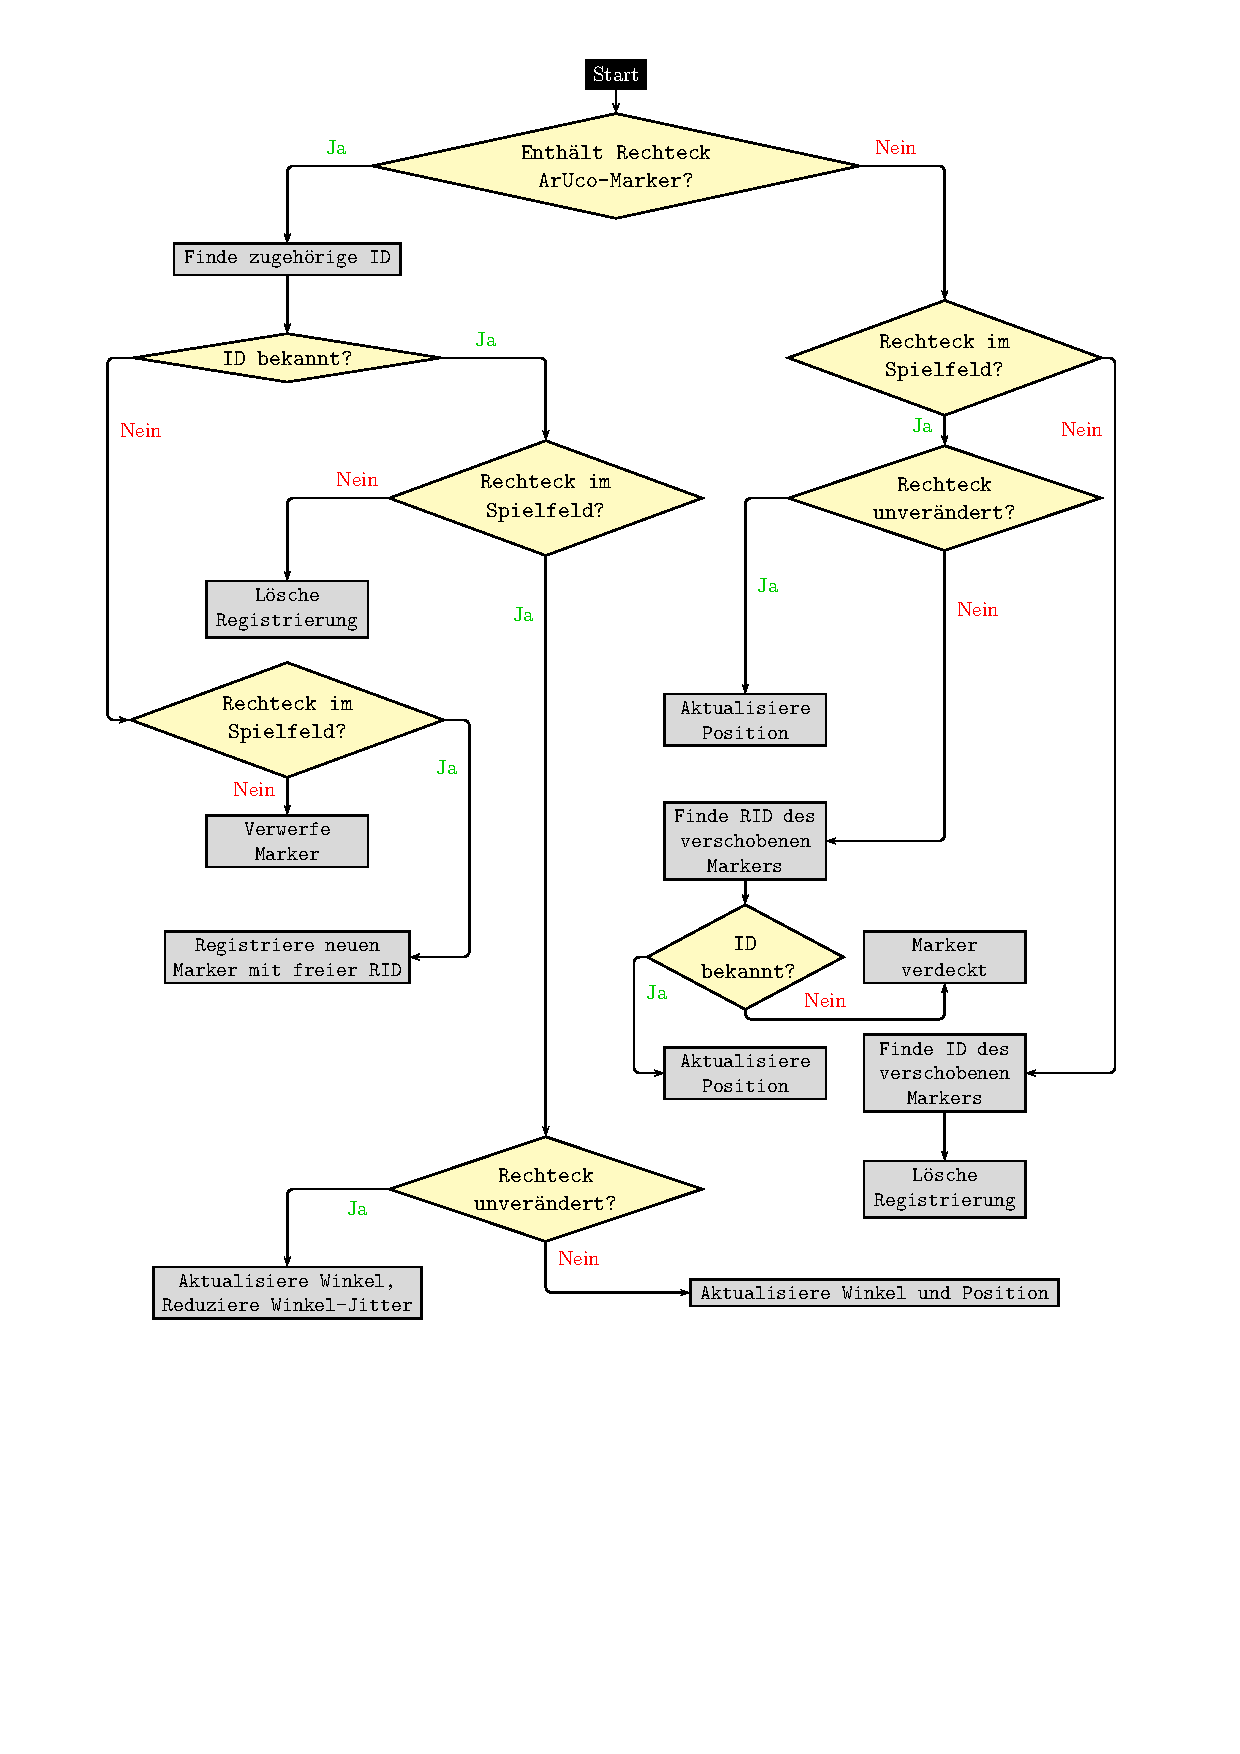
\includegraphics[scale=.8, trim=3cm 2.5cm 3.5cm 9 cm]{kapitel/system/MP_Marker_Erkennung.pdf}
	\caption{Flussdiagramm des Marker Trackings.}
	\label{fig:TrackingDiagram}
\end{figure}

Im Folgenden wird auf die Implementierung der Funktionen zum Marker Tracking eingegangen. Diese werden von der Klasse \texttt{IdMapping.cpp} zur Verfügung gestellt und in der Methode \texttt{track\-Marker()} aufgerufen.
\begin{itemize}
\item \texttt{is\-Constant\-Marker()} prüft ob die Position $p_c$ eines Markers unverändert ist und gibt die ermittelte RID zurück. Indem die Länge $\|v_m\|$ aller Bewegungsvektoren berechnet wird und prüft ob $\|v_m\|\le 3$ Pixel ist. Mit anderen Worten gilt ein Marker als unverändert, wenn sich $p_c$ innerhalb einer $3 \times 3$ Nachbarschaft \textcolor{red}{Besser Pixelnachbarschaft?} bewegt. Diese Toleranz ist notwendig, da es durch das Bildrauschen zu geringfügigen Abweichungen kommen kann.
\item \texttt{is\-Translated\-Marker()} hat die Aufgabe Marker zu finden, die bewegt wurden. Hier wird die Zuordnung auch innerhalb eines Bewegungsradius von $100$ Pixeln mit Hilfe von $\|v_m\|$  abgeschätzt. Diese Art des Trackings kann unter Umständen zu einer falschen Zuordnung führen. Doch der große Vorteil ist der gering Kostenaufwand und mit Betrachtung der Umstände sinkt die Wahrscheinlichkeit einer Fehlinterpretation auf ein vertretbares Risiko. Bei einem dieser Umstände handelt es sich um die Annahme das ein Nutzer nur maximal zwei Marker zum gleichen Zeitpunkt bewegen wird, während alle weiteren unbewegten Marker vorab als unverändert eingestuft wurden und nicht mehr während der aktuellen Iteration berücksichtigt werden.\\
Ein anderer Fakt ist, dass durch die Verwendung der \textit{ArUco} Marker zu jedem Zeitpunkt ein Marker wieder eindeutig zu geordnet werden kann. Dies ist unter anderem der Fall, wenn angenommen wird, dass der Markercode nur langsam in der näheren Umgebung anderer Würfel Marker bewegt wird. Nach erfolgreichem Tracking wird die ermittelte RID zurückgeben.
\item \texttt{isMarker\-Out\-OfField()} und \texttt{is\-Rect\-Out\-Of\-Field()} testen ob sich das OBB noch innerhalb des rechteckigen Arbeitsbereichs befindet. Dieser Arbeitsbereich ist vom Typ \texttt{Rect} der \textit{OpenCV} Bibliothek, welcher die Funktion \texttt{contains} implementiert. Hier wird geprüft, ob ein übergebener Punkt innerhalb des bei der Kalibrierung aufgespannten Rechtecks liegt. \texttt{isMarker\-OutOf\-Field()} kann bei bekannter RID ein gesamtes Markerobjekt übergeben bekommen und \texttt{isRectOutOfField} verlangt ein \text{RotatedRect} als Übergabeparameter.
\item \texttt{hasArucoID()} teilt jeweils die vier Punkte des Vierecks vom \textit{ArUco}-Marker in zwei Dreiecke auf und mit beiden wird ein \text{Punkteinschlusstest} mit Baryzentrischen Koordinaten durchgeführt \cite{article:BaryzentriFarin}. Liegt der Schwerpunkt eines OBB in einem der beiden Dreiecke umschließt das Rechteck einen \textit{ArUco}-Marker. Bei diesem Test werden die Vorzeichen der Koordinaten betrachtet, denn ein Punkt liegt im Dreieck falls alle Vorzeichen gleich oder null\textcolor{red}{Vorzeichen können nicht null sein:P} sind liegt der Punkt im Dreieck. Der Vorteil dieses Tests ist, dass er mit wenigen kostenarmen Skalarprodukten und einfachen arithmetrischen Berechnungen durchführbar ist und somit die Performanz des Tracking Algorithmus wenig beeinflusst. 
\end{itemize}
Im Anschluss eines erfolgreichen Marker Trackings müssen alle $p_c$ der registrierten Marker vom zweidimensionalen Bildraum in die dreidimensionale \textit{Unity}-Welt transformiert werden. Die erste Transformation schätzt die Position von $p_c$ im dreidimensionalen Kameraraum ab. Dieser \texttt{tvec} wird mit der Funktion \texttt{estimate\-Pose\-Single\-Markers()} des \textit{OpenCV} Moduls \texttt{aruco} abgeschätzt.
Das Ergebnis dieser Schätzung ist der Transformationsvektor $v_t$ \textcolor{red}{bei mir heißt der $t$}, welcher anschließend mit der affinen Transformationsmatrix $T_aff$ \textcolor{red}{heißt bei mir $M_{affin}$}in die \text{Unity}-Welt verschoben wird (vgl. Abschnitt~\ref{sec:planeCalib}). Der letzte Schritt wird in der Klasse \texttt{Coords\-Trans\-formtion\-2Untiy.cpp} \textcolor{red}{Falsch geschrieben??} mit der Methode \texttt{computeTransformation2Unity} durchgeführt indem $v_t$ mit $T_aff$ \textcolor{red}{Bei mir $t$ und $M_{affin}$}multipliziert wird. Zu diesem Zeitpunkt werden die relevanten Daten der Marker Objekte per TCP an den \textit{Unity}-Computer übertragen. Die Übertragung wird in der Klasse \texttt{TCP.cpp} aufgebaut und gesteuert. Nach erfolgreicher Übertragung beginnt eine neue Iteration (siehe Kapitel \ref{sec:serverClient}).

\newpage